\documentclass{article}

\usepackage[dutch]{babel}
\usepackage[margin=3cm]{geometry}
\usepackage{graphicx}
\usepackage{float}
\usepackage{caption}
\usepackage{hyperref}
\usepackage{amsmath}
\usepackage{wrapfig}
\usepackage[parfill]{parskip}

% fonts
\usepackage[T1]{fontenc}
\usepackage{helvet}
\renewcommand{\familydefault}{\sfdefault}

\graphicspath{{img/}}
 
\newcommand{\bold}[1]{\textbf{#1}}

%Define the listing package
\usepackage{listings} %code highlighter
\usepackage{upquote}
\usepackage{color} %use color
\definecolor{mygreen}{rgb}{0,0.6,0}
\definecolor{mygray}{rgb}{0.5,0.5,0.5}
\definecolor{mymauve}{rgb}{0.58,0,0.82}

\begin{document}

\begin{titlepage}
    \author{Tuur Vanhoutte}
    \title{IoT Cloud}
\end{titlepage}

\pagenumbering{gobble}
\maketitle
\newpage
\tableofcontents
\newpage

\pagenumbering{arabic}

\section{Cloud computing}

= the practice of using a network of remote servers hosted on the Internet to store, manage, and process data, rather than a local server or a personal computer.

\subsection{Enkele eigenschappen}
\begin{itemize}
    \item Geen eigen hardware (we kopen niets aan)
    \item Ongelimiteerde computing power
    \item Ongelimiteerde storage capaciteit
    \item Scaling up and down op aanvraag of
    automatisch
    \item Scaling in en out op aanvraag of
    automatisch
    \item Geografische spreiding
    \item Pay what you use
\end{itemize}

\begin{figure}[H]
    \centering
    \includegraphics[width=0.7\textwidth]{cloud-hosting.png}
    \caption{}
\end{figure}


\subsection{On premise (eigen servers)}

\begin{itemize}
    \item IT Afdeling is verantwoordelijk voor ALLES
    \item Back-up \& recovery
    \item Aankoop hardware
    \item Scaling...
    \item Meeste vrijheid om te werken
    \item Soms investeren in hardware die je maar beperkt aantal dagen nodig hebt
    \item Vb: webshop en kerstperiode
    \item Soms verplicht door wetgeving
    \item Medische data
    \item Financial data
    \item Gebrek aan vertrouwen bij public cloud provider (cfr NSA)
\end{itemize}

\subsection{Hybrid Cloud (On Premise \& Cloud)}
Makes use of existing in-house infrastructure and Netplan cloud services to provide the best of both worlds.

\begin{itemize}
    \item Eigen datacenter koppelen aan cloud omgeving
    \item Bepaalde diensten draaien in cloud omgeving andere in eigen datacenter
    \item Zware load laten uitvoeren op de cloud
    \item Bepaalde data mag NIET in cloud opgeslagen worden vb: medical
    \item Kan ook gebruikt worden in back-up scenario’s
\end{itemize}

\subsection{IaaS: Infrastructure as a Service}

\begin{itemize}
    \item Geen eigen hardware kopen
    \item We huren virtual machines in Cloud omgeving
    \item Systeem beheerder moet zelf server configureren en beveiligen en updaten
    \item Veel flexibiliteit naar software installatie toe
    \item Zeer veel vrijheid maar ook verantwoordelijkheid
    \item Je moet zelf scaling doen (soms auto scaling mogelijk)
    \item Veel gebruik voor migratie bestaande On Premise naar cloud
\end{itemize}

\subsubsection{Voorbeelden}
\begin{itemize}
    \item Amazon Web Services (AWS)
    \item Microsoft Azure
    \item IBM Bluemix
    \item Google Cloud platform
\end{itemize}

\subsection{PaaS: Platform as a Service}

\begin{itemize}
    \item Geen systeembeheerder nodig
    \item Ontwikkelaar maakt applicatie en "plaatst" deze op Cloud platform
    \item We moeten ons geen zorgen maken in servers, hosting, back-ups, scaling,... het platform zal dit voor ons beheren
    \item Zeer veel flexibiliteit
\end{itemize}

We zullen vooral dit gebruiken in IoT Cloud module.

\subsubsection{Talen}
\begin{itemize}
    \item ASP.NET Core
    \item NodeJS
    \item Python
    \item Java
    \item PHP
\end{itemize}

\subsubsection{Voorbeelden}
\begin{itemize}
    \item Amazon Web Services (AWS)
    \item Microsoft Azure
    \item IBM Bluemix
    \item Google Cloud platform
    \item Heroku
\end{itemize}

\subsection{SaaS}
\begin{itemize}
    \item Software draait meestal niet lokaal (uitzondering Adobe \& Office)
    \item We betalen per maand/gebruiker
    \item Flexibele abonnementen, snel op te zetten
    \item We moeten geen rekening houden met back-ups en uptime
\end{itemize}

\subsubsection{Voorbeelden}
\begin{itemize}
    \item salesforce
    \item Office 365
    \item Dropbox, OneDrive, Google Drive, iCloud
    \item Gmail
    \item Adobe Creative Cloud
\end{itemize}

\subsection{Belangrijkste vendors}
\begin{itemize}
    \item Amazon Web Services
    \item Microsoft Azure
    \item Google Cloud Platform
\end{itemize}

\begin{figure}[H]
    \centering
    \includegraphics[width=0.5\textwidth]{magic-quadrant.png}
    \caption{}
\end{figure}



\section{Microsoft Azure}
We kiezen voor Microsoft Azure omwille van:
\begin{itemize}
    \item Zowel .NET als Open Source (PHP, Java, Node, Python, Flask, Docker...)
    \item Meeste opties en mogelijkheden
    \item Zeer lage instapdrempel voor studenten
\end{itemize}


\subsection{Azure Portal}

Inloggen via \url{portal.azure.com}

\begin{itemize}
    \item Beheren van uw Cloud services en applicaties
    \item Inloggen met Howest Account
    \item Kies een voldoende sterk passwoord en gebruik 2FA
\end{itemize}

\subsection{Azure subscription}
\begin{itemize}
    \item Abonnement
    \item Dit zal bepalen hoe ze factureren
    \item Verschillende opties:
    \begin{itemize}
        \item Credits op voorhand
        \item Pay by use
    \end{itemize}
    \item In de praktijk: per klant een subscription
    \item Voor de lessen: we hebben de "gratis subscription"
    \item Meerdere subscriptions mogelijk
\end{itemize}

\subsection{Resource Group}

\begin{figure}[H]
    \centering
    \includegraphics[width=0.5\textwidth]{resource-group.png}
    \caption{Resource groups}
\end{figure}

\begin{itemize}
    \item Logische container
    \item Per project
    \item Per soort services
    \begin{itemize}
        \item Storage
        \item Webservers
        \item Fileservers
        \item SQL, Blob, \dots
    \end{itemize}
    \item Je kiest dit zelf
    \item Makkelijk om te testen, je kan een volledige container verwijderen zonder dat je alles apart moet verwijderen
    \item Toegangsrechten per container zijn mogelijk
    \begin{itemize}
        \item via Office 365 account
    \end{itemize}
    \item Je kies datacenter locatie van je resource group, niet alle resources moeten op dezelfde locatie staan als je resource group.
\end{itemize}

\subsection{Azure Virtual Machines}
\begin{itemize}
    \item Eigen server op Azure omgeving
    \item Meestal on-premise (server op bedrijf) die we virtueel verplaatsen naar Azure
    \item Heel wat mogelijkheden
    \begin{itemize}
        \item File servers
        \item Database servers
        \item Webservers
        \item Application servers
        \item ...
    \end{itemize}
    \item Toegang tot resources op server die niet mogelijk zijn via een web applicatie
    \begin{itemize}
        \item Bv. communicatie met oude software pakketten
        \item Bv. Genereren van Word/Excel documenten
        \item \dots
    \end{itemize}
\end{itemize}

\subsubsection{Waarom?}
Wanneer je volledige controle wenst over je machine

\begin{itemize}
    \item Volledige controle == volledige verantwoordelijkheid!
    \begin{itemize}
        \item Niet te onderschatten
        \item Security, patching, scaling
    \end{itemize}
    \item Windows
    \item Linux
\end{itemize}

\subsubsection{Maintenance}

\begin{itemize}
    \item Planned maintenance
    \begin{itemize}
        \item Updates van het Azure platform (stabiliteit, security, performance)
        \item Soms moet de VM herstarten
    \end{itemize}
    \item Unplanned maintenance
    \begin{itemize}
        \item Storing in de onderliggende architectuur (netwerk-, disk-, rack-problemen)
        \item Azure zal automatisch VM verplaatsen naar werkende infrastructuur
    \end{itemize}
\end{itemize}

Hoe kan ik mijn VM `up and running' houden?
\begin{itemize}
    \item Availability set
    \begin{itemize}
        \item Garantie van 99.95\% uptime
        \item Minstens 2 virtual machines nodig
        \item Duurder
    \end{itemize}
\end{itemize}

\subsection{Azure Web App}
\begin{itemize}
    \item Azure Platform Service
    \item Laat ons toe om webapps online te plaatsen
    \item We moeten GEEN eigen server aanmaken
    \item We moeten GEEN webserver configureren
    \item Click \& go
    \item Ondersteuning voor:
    \begin{itemize}
        \item ASP.NET (Core)
        \item PHP
        \item Python Flask
        \item Java
        \item Node.JS
        \item \dots
    \end{itemize}
    \item Makkelijkste manier om uw applicatie online te krijgen, easy deployment
    \item Eenvoudige te koppelen aan een GitHub Repository
    \item Autoscale (not free)
    \item Monitoring
    \item Staging mode
\end{itemize}

\subsubsection{Free}
= gratis plan voor Azure Web App

\begin{itemize}
    \item Gedeelde server met andere web apps
    \item Je weet niet welke server, is transparant voor gebruiker
    \item 1GB storage
    \item Beperking op trafiek per dag: 165MB
\end{itemize}

\subsubsection{Shared}
\begin{itemize}
    \item Gedeelde server
    \item 1GB storage
    \item Mogelijkheid tot DNS vb: www.mijnnaam.be
\end{itemize}

\subsubsection{Basic, Premium}
\begin{itemize}
    \item App service plan $\Rightarrow$ eigen server, dus niks delen met derden (je kan niet inloggen op die server)
    \item SSL
    \item Custom domains
    \item CPU keuze
    \item Memory keuze
    \item Scaling tot 3 toestellen
\end{itemize}

\subsection{Scaling}

\subsubsection{Scale Up}
\begin{itemize}
    \item = vertical scaling
    \item Server krachtiger maken, meer memory en CPU
\end{itemize}

Pros: 
\begin{itemize}
    \item Minder energie dan scale out
    \item Eenvoudiger te implementeren
    \item Minder licenties (n.v.t. op Azure Web App)
\end{itemize}

Cons:

\begin{itemize}
    \item Duurder
    \item Indien we maar 1 machine gebruiken: $\Rightarrow$ hardware failure en toepassing is down
\end{itemize}


\subsubsection{Scale Out}
\begin{itemize}
    \item = horizontal scaling
    \item Meerdere machiens maar minder krachtig
\end{itemize}

Pros: 
\begin{itemize}
    \item Goedkoper
    \item Betere bescherming bij hardware failure, hebt meerdere machines
\end{itemize}

Cons:

\begin{itemize}
    \item Meer licenties nodig (n.v.t. op Azure)
    \item Meer plaats in datacenter
    \item Meer energieverbruik
    \item Complexer netwerk
    \item Soms toepassing aanpassen
\end{itemize}

\subsection{Azure SQL}

\begin{itemize}
    \item 
    \item SQL Server Database op Cloud platform
    \item We moeten zelf geen hardware/software aankopen
    \item Niet verantwoordelijk voor backups
    \item Eenvoudige schalen bij zware loads
    \item 3 opties
    \begin{itemize}
        \item Serverless Managed Database (onze voorkeur)
        \item SQL Managed Instance
        \item SQL Virtual Machine
    \end{itemize}
\end{itemize}

\subsubsection{SQL Server Cloud Based}
\begin{itemize}
    \item Compatible met SQL server 2012
    \item Te beheren via Enterprise manager
    \item Werkt zoals een gewone SQL server
    \item Connecteren is mogelijk via:
    \begin{itemize}
        \item .NET
        \item Python
        \item PHP
        \item Node
        \item \dots
    \end{itemize}
    \item High Availability
    \begin{itemize}
        \item Replicatie over 3 servers (default)
        \item Automatische Back-ups
    \end{itemize}
    \item Database draait op een server
    \item Verschillende pricing mogelijkheden
\end{itemize}

\subsubsection{Eigenschappen}
\begin{itemize}
    \item Database draait op een server
    \item Verschillende pricing mogelijkheden
\end{itemize}

\subsubsection{Security}
Azure FireWall: IP adres van je netwerk toelaten

\subsubsection{Azure DTU}
\begin{itemize}
    \item DTU = Database Transaction Units
    \item Soort `munteenheid'
    \item Gemengde eenheid van:
    \begin{itemize}
        \item CPU
        \item Memory
        \item I/O
    \end{itemize}
    \item Deze resources krijg je ter beschikking
    \item Hoe meer DTU, hoe meer power, hoe duurder
    \item \url{https://docs.microsoft.com/en-us/azure/sql-database/sql-database-what-is-a-dtu}
    \item vCores = virtuele CPUs die de service mag gebruiken
\end{itemize}

\subsubsection{Throttling}
= Onderbreken van database communicatie omdat je teveel resources (DTU's) gebruikt (zelf voor retry zorgen).

\begin{figure}[H]
    \centering
    \includegraphics[width=0.8\textwidth]{azure-throttling.png}
    \caption{Throttling types}
\end{figure}

\begin{figure}[H]
    \centering
    \includegraphics[width=0.8\textwidth]{azure-throttling-modes.png}
    \caption{Throttling modes}
\end{figure}

\begin{figure}[H]
    \centering
    \includegraphics[width=0.8\textwidth]{azure-sql-command-ex.png}
    \caption{Voorbeeld SQL command in C\#}
\end{figure}


\subsubsection{Resources}
\begin{itemize}
    \item \url{https://msdn.microsoft.com/en-us/library/azure/dn338079.aspx}
    \item \url{http://geekswithblogs.net/ScottKlein/archive/2012/01/27/understanding-sql-azure-throttling-and-implementing-retry-logic.aspx}
\end{itemize}

\subsubsection{Azure Database for MySQL}

\begin{itemize}
    \item Toegang via MySQL Workbench
    \item Werkt zoals een gewone MySQL DB
    \item Je moet geen eigen servers opzetten, is volledig managed
    \item Automatische Back-ups
\end{itemize}

\subsection{Azure \& Internet of Things}

\subsubsection{Waarom is Azure belangrijk voor IoT?}

\begin{itemize}
    \item Azure Event Hubs
    \begin{itemize}
        \item Ontvangen van berichten afkomstig van toestellen
    \end{itemize}
    \item \textcolor{red}{Azure IoT Hub}
    \begin{itemize}
        \item Ontvangen van berichten
        \item Versturen van berichten naar toestellen
    \end{itemize}
    \item Azure Streaming Analytics
    \begin{itemize}
        \item Verwerken van events afkomstig van Event Hubs en IoT Hub
    \end{itemize}
\end{itemize}

\bold{Bovenstaande zeer belangrijk voor ons!}

\begin{figure}[H]
    \centering
    \includegraphics[width=0.8\textwidth]{azure-iot-microsoft-services.png}
    \caption{Microsoft Services}
\end{figure}

\subsection{Azure CLI}

\subsubsection{Azure Portal}

\begin{itemize}
    \item OK voor dagelijks gebruik
    \item Niet makkelijk te automatiseren
    \item Wat als ik 100 sites nodig heb?
    \item Wat als ik 50 servers nodig heb?
\end{itemize}

\subsubsection{Oplossing: Azure CLI 2.0}
\begin{itemize}
    \item Commandline Azure resources aanmaken
    \item Makkelijk met scripts
    \item Ideaal voor DevOps
\end{itemize}

\subsection{Bash/Powershell}

\begin{itemize}
    \item Bash commandline in portal
    \item Alles wat je via UI kan doen kan je ook via commandline in de portal
\end{itemize}

\subsection{Andere Azure onderdelen}
\begin{figure}[H]
    \centering
    \includegraphics[width=0.95\textwidth]{azure-onderdelen.png}
    \caption{}
\end{figure}

\subsection{Samenvatting}
\begin{itemize}
    \item Wat is Cloud computing?
    \item Wie zijn de grote spelers?
    \item Welke soorten zijn er en wat zijn hun eigenschappen?
    \item Wat is een Azure subscription?
    \item Wat zijn resource groups?
    \item Hoe kan je scalen?
    \item Voor en nadelen van Azure VM’s?
    \item Wanneer Azure VM gebruiken?
    \item Wat is SQL Azure en wat zijn DTU’s?
    \item Wat is throttling?
    \item Wat is een Azure Web App?
\end{itemize}

\section{Back-end services met Azure functions}

\subsection{The Internet of \dots}

\subsubsection{The Internet of Information}
\begin{itemize}
    \item Het draait om webpagina’s met content
    \begin{itemize}
        \item Opzoeken van informatie
        \item Raadplegen van informatie
        \item E-commerce
        \item Social networks
    \end{itemize}
    \item Technologie
    \begin{itemize}
        \item HTML
        \item CSS
        \item JavaScript
        \item PHP/ASP/JAVA
    \end{itemize}
    \item Voorbeelden
    \begin{itemize}
        \item Google
        \item Facebook
        \item Amazon
        \item Stackoverflow
        \item Nieuwssites
    \end{itemize}
\end{itemize}


\subsubsection{The Internet of Services}
\begin{itemize}
    \item Connectiviteit
    \begin{itemize}
        \item Driving factor mobile applications
        \item Cross platform
        \item Data op makkelijke manier uitwissen
        \item Functionaliteit makkelijk aanroepen
        \item Centraal staan Cloud platforms
        \item REST Based
    \end{itemize}
    \item Voorbeelden
    \begin{itemize}
        \item Netflix
        \item Azure
        \item Amazon Web Services (AWS)
        \item IBM Bluemix
    \end{itemize}
\end{itemize}


\subsubsection{The Internet of Things}
= Connecting hardware

\begin{itemize}
    \item Device koppelen aan het internet
    \begin{itemize}
        \item Versturen van informatie naar cloud
        \item Toestellen praten onderling met elkaar (M2M = machine to machine)
    \end{itemize}
    \item Communicatie van/naar toestel
    \begin{itemize}
        \item We kunnen berichten sturen naar toestel
        \item We ontvangen berichten van toestel in de cloud
    \end{itemize}
    \item Voorbeelden
    \begin{itemize}
        \item Smart thermostat
        \item Smart fridge
        \item Auto's die verbonden zijn met de cloud (Tesla)
        \item Andere smart home devices (Alexa, \dots)
    \end{itemize}
\end{itemize}

Internet of Things \& Internet of services overlappen

\subsubsection{Volgende stap: The Internet of Value}

"Value" verhandelen via het internet

\begin{itemize}
    \item Bitcoin
    \item Andere cryptocurrencies
\end{itemize}

Onderliggende technologie veel belangrijker: Blockchain

\begin{itemize}
    \item Distributed ledger (grootboek)
    \item Registreren van transacties in die ledger
    \item Iedere transactie bevat een verwijzing naar de vorige transacties (chain, linked list)
\end{itemize}

\bold{Blockchain}
\begin{itemize}
    \item Public
    \item Gratis
    \item Open
\end{itemize}

\begin{itemize}
    \item Private blockchain mogelijk
    \begin{itemize}
        \item Veel evolutie in de wereld van de fintech
        \item Etherium
        \item Smart contracts
    \end{itemize}
    \item IoT \& blockchain zeer veel potentieel
    \item Bachelor-proef (project 4)
\end{itemize}

\begin{figure}[H]
    \centering
    \includegraphics[width=0.6\textwidth]{gartner-hype-cycle.png}
    \caption{}
\end{figure}

Onze focus: Internet of Things \& Internet of Services

\subsection{Herhaling: Hoe werkt HTTP?}
\begin{figure}[H]
    \centering
    \includegraphics[width=0.5\textwidth]{osi.png}
    \caption{HTTP staat op OSI laag 7: de application layer}
\end{figure}

\begin{figure}[H]
    \centering
    \includegraphics[width=0.5\textwidth]{http-website.png}
    \caption{Hoe werkt een website?}
\end{figure}


\subsubsection{Wat is HTTP?}
\begin{itemize}
    \item Hyper Tekst Transfer Protocol
    \item Onderliggende protocol waarop Internet werkt
    \item Opvragen van tekst, bestanden vanaf servers
    \item Request \textit{meestal} afkomstig van een webbrowser maar ook smartphone, IoT device
    \item HTTP zal bepalen hoe een request en response er moeten uitzien
    \item HTTP bevat een aantal commando’s: \bold{HTTP Verbs}
    \item HTTP is \bold{stateless}, het zal dus geen rekening houden met voorgaan requests ("Fire and Forget")
    \item HTTP is \bold{niet sessionless}, we kunnen cookies (client-side) gebruiken om data bij te houden
    \item HTTP is relatief eenvoudig: volledig text-based
\end{itemize}

\subsubsection{HTTP Verbs}
= HTTP commands/methods

\begin{itemize}
    \item \bold{GET} - ophalen data (safe: wijzigt niets op server) (SELECT)
    \item \bold{POST} - Toevoegen data: vb: formulier (INSERT)
    \item \bold{PUT} - Idempotent => meerdere requests => zelfde effect (UPDATE)
    \item \bold{DELETE} - Idempotent => meerdere requests => zelfde effect (DELETE)
\end{itemize}

\subsubsection{HTTP status code}
HTTP Response bevat naast data (html of andere) ook een status code: 

\begin{itemize}
    \item 1xx: informatief
    \item 2xx: success
    \item 3xx: redirection
    \item 4xx: client error
    \item 5xx: server error
\end{itemize}

Niet altijd evident om te weten wat je moet kiezen !

\subsubsection{HTTPS}

\begin{itemize}
    \item Beveiligen van transport
    \item Geen beveiliging van de data
    \item Defacto standaard, zonder HTTPS mag je eigenlijk \bold{niet} in productie plaatsen
    \item Browsers melden dit reeds, vb:Chrome
\end{itemize}

\begin{figure}[H]
    \centering
    \includegraphics[width=0.3\textwidth]{https.png}
    \caption{HTTPS info in Google Chrome. Hier: geen HTTPS verbinding, enkel HTTP}
\end{figure}

\subsubsection{HTTP Request}
\begin{figure}[H]
    \centering
    \includegraphics[width=0.8\textwidth]{http-request.png}
    \caption{HTTP GET-Request}
\end{figure}

\begin{itemize}
    \item Belangrijkste HTTP Header info: User-Agent zal dit opstellen
    \item GET = HTTP verb
    \item Host = de server
    \item User-Agent = browser info
    \item Accept = welke type data kan de client ontvangen
\end{itemize}

\subsubsection{HTTP Response}
\begin{figure}[H]
    \centering
    \includegraphics[width=0.5\textwidth]{http-response.png}
    \caption{HTTP Response met status code 200}
\end{figure}

\begin{itemize}
    \item Belangrijkste HTTP Header info: Server zal dit opstellen
    \item 200 OK = status code
    \item Content-Type = wat is het type van de info die ik ontvang, vb text/html
    \item Inhoud resource: vb: HTML code
\end{itemize}

\subsubsection{HTTP/2}

\begin{itemize}
    \item Sinds 2015 actief
    \item High-Level compatibility met HTTP/1.1 - methods, status codes, URI's en Header fields zijn hetzelfde
    \item Request multiplexing over een enkele TCP verbinding
    \begin{itemize}
        \item Meerdere request in parallel mogelijk over 1 tcp connection
        \item Asychroon downloaden van meerdere bestanden mogelijk
    \end{itemize}
    \item Header compression (optimalisatie van het netwerk)
    \item Binary Protocol (HTTP/1.1 is tekst protocol)
    \item HTTP/2 Server push: staat een HTTP/2-server toe om resources te sturen naar een HTTP/2-compatibele client voor de client ze vraagt (=performancetechniek)
\end{itemize}


\subsection{Webservices}
= functies die we kunnen aanroepen via het internet

\begin{itemize}
    \item Opvragen van data via het internet
    \item Devices aanspreekbaar maken via het internet
    \item Protocol is default (HTTP)
    \item Technologie-onafhankelijk (Java, C\#, PHP, Python)
    \item Platform-onafhankelijk (Windows, Linux, Android, iOS)
    \item 2 Protocollen:
    \begin{itemize}
        \item SOAP (verouderd, meestal gebruikt tss 2000-2010, gebruiken wij niet)
        \item REST (onze keuze)
    \end{itemize}
    \item Datatransport (formaat van de data) via
    \begin{itemize}
        \item XML
        \item JSON
    \end{itemize}
\end{itemize}

\subsubsection{Open data}
= data die vrij beschikbaar is

\begin{itemize}
    \item Opvraagbaar via webservices
    \item Meer en meer steden stellen data beschikbaar:
    \begin{itemize}
        \item Gent: \url{https://data.stad.gent/}
        \item Federale overheid: \url{http://data.gov.be/en}
    \end{itemize}
\end{itemize}

\subsubsection{Cognitive services}
\begin{itemize}
    \item = AI API op Azure
    \begin{itemize}
        \item \url{https://azure.microsoft.com/en-us/services/cognitive-services/}
        \item Spraak
        \item Beeldherkenning
        \item Taal
        \item \dots
    \end{itemize}
\end{itemize}

\subsubsection{Internet of Things}
\begin{itemize}
    \item Philips Hue API (\url{http://developers.meethue.com/)})
    \item Parrot AR Drone (\url{https://github.com/andrew/ar-drone-rest})
\end{itemize}

Alle voorgaande voorbeelden:
\begin{enumerate}
    \item Maken gebruik van HTTP
    \item GET/POST request naar device
    \item In de body van het request: JSON data
    \item Cross-platform
\end{enumerate}

Deze manier van werken zal je ongeveer altijd tegenkomen!

\subsubsection{JSON}

\begin{itemize}
    \item Het meest gebruikte formaat voor data is XML en JSON (wij kiezen voor JSON)
    \item De data die je terugkrijgt zal altijd mappen met een object aan de serverkant
\end{itemize}

\bold{JSON = JavaScript Object Notation}

\begin{itemize}
    \item Eenvoudig, zeer licht formaat
    \item We schrijven alles tussen accolades
    \item Basis is altijd key:value pair
    \begin{itemize}
        \item De key = lowercase, altijd tussen quotes
        \item Value: indien string $\Rightarrow$ quotes
        \item Key en value geschieden door een dubbelpunt :
        \item Key:value koppels geschieden door een komma ,
    \end{itemize}
    \begin{itemize}
        \item Validatie en testen kan op \url{https://jsonlint.com/}
    \end{itemize}
\end{itemize}

\bold{Complexe JSON}

\begin{itemize}
    \item Een key kan als value terug een JSON string bevatten
    \item Daarbinnen kan je terug een key plaatsen met een nieuwe JSON string
    \item Je kan zoveel nesten als je wil.
\end{itemize}

\bold{Complexe JSON Arrays}

\begin{itemize}
    \item Wanneer er meerdere JSON objecten zijn spreken we van een array
    \item Deze plaatsen we tussen []
    \item Een key kan terug als value een array van andere JSON objecten zijn
\end{itemize}

\subsubsection{URL}
\begin{itemize}
    \item Alles is uniek identificeerbaar via een URL $\Rightarrow$ Uniform Resource Locator
    \item Gebruik \bold{geen} spaties in de URL
    \item Gebruik \bold{geen} hoofdletters
    \item Gebruik meervoud voor resource namen
    \item Gebruik GEEN HTTP Verb om operatie aan te duiden (vb: geen get of post in url)!!
\end{itemize}

Voorbeelden 

\begin{itemize}
    \item \url{http://localhost:8080/UserManagement/rest/UserService/getUser/1} 
    \begin{itemize}
        \item NIET OK: operatienaam in URL en hoofdletters
    \end{itemize}
    \item \url{http://localhost:8080/usermanagement/rest/userservice/users/1} 
    \begin{itemize}
        \item OK: resourcenaam = meervoud, gevolgd door ID van de user die we willen opvragen
    \end{itemize}
\end{itemize}

\subsubsection{Fouten}
Wat als er iets foutloopt in een service?

\begin{itemize}
    \item Wat moet ik terugkeren ?
    \item Stuur NOOIT maar dan ook NOOIT Exceptions of intern foutmeldingen van het systeem terug naar de client in productie systemen
    \item Keer een status code Internal Sever Error 500 terug met eventueel wat informatie die jij opstelt
    \item Denk na welke info je bij de foutmelding wil terugsturen
    \begin{itemize}
        \item Geen connectie informatie
        \item Geen database namen
        \item Geen SQL statements
        \item Wees voorzichtig\dots
    \end{itemize}
\end{itemize}

\subsubsection{Samenvatting}
\begin{itemize}
    \item HTTP GET
    \begin{itemize}
        \item Alleen lezen (SELECT in database)
    \end{itemize}
    \item PUT \& DELETE
    \begin{itemize}
        \item DELETE = DELETE in SQL
        \item PUT = UPDATA in database
        \item Idempotent methodes $\Rightarrow$ voer je ze 1x uit of 100x, het resultaat blijft hetzelfde
    \end{itemize}
    \item HTTP POST
    \begin{itemize}
        \item INSERT in SQL
    \end{itemize}
\end{itemize}

\bold{Webservices zijn stateless}

\begin{itemize}
    \item Geen state van de client bijhouden aan serverkant
    \item Geen sessies gebruiken
    \item Bij iedere request naar de server moet ja alle info meesturen zodat server het request kan afhandelen
    \item Ieder request is onafhankelijk van elkaar
    \item Dit verhoogt de schaalbaarheid
    \item Eenvoudiger applicatie design
    \item Vb: vanuit een mobile app vragen we sensor data op via webservice. 
    De gebruiker van de app kan een filter instellen en wil enkel de temperatuur sensor data zien. 
    Dit wil zeggen bij iedere request naar de server MOET je meegeven welke data de gebruiker wil zien. 
    Je mag aan de server kant NIET bijhouden welke gebruiker welke sensors data wenst te zien
\end{itemize}

\subsubsection{Hoe maken we webservices?}

\begin{itemize}
    \item Aanwezig op ieder platform
    \item PHP
    \begin{itemize}
        \item Laraval, Lumen, Wave
    \end{itemize}
    \item Python
    \begin{itemize}
        \item Eve, Flask-Restfull
    \end{itemize}
    \item .NET
    \begin{itemize}
        \item ASP.NET Core met C\#
        \item Azure Functions
        \begin{itemize}
            \item Met C\#, NodeJS of Python
        \end{itemize}
    \end{itemize}
\end{itemize}

\subsection{Azure Functions}
= Serverless functions 

\subsubsection{Waarom?}
\begin{itemize}
    \item Eenvoudig concept, zeer eenvoudig aan te maken
    \item Ondersteuning voor verschillende talen
    \begin{itemize}
        \item Wij gebruiken C\# maar Python kan ook: \url{https://docs.microsoft.com/en-us/azure/azure-functions/functions-reference-python}
    \end{itemize}
    \item Snel en eenvoudig schaalbaar
    \item Geen zorgen over servers en serverbeheer (serverless)
\end{itemize}

\subsection{Azure Functions security}
\begin{itemize}
    \item Iedereen kan functies aanspreken
    \item Geen controle over wie wat doet
    \item Een hacker kan de factuur doen oplopen door constant de service aan te roepen
    \item Andere normale gebruikers zullen tragere API aanroepen krijgen
    \item Concreet: we moeten dit proberen te vermijden
\end{itemize}

3 soorten security

\begin{enumerate}
    \item Anonymous
    \begin{itemize}
        \item Iedereen kan de functie aanroepen
    \end{itemize}
    \item Function
    \begin{itemize}
        \item Er zal een function key meegegeven worden via de URL
        \item Deze key kan alleen gebruikt worden bij de gekozen functie
    \end{itemize}
    \item Admin 
    \begin{itemize}
        \item De admin key zal mee moeten verstuurd worden via de URL
        \item Deze key kan gebruikt worden voor alle functies binnen de applicatie
    \end{itemize}
\end{enumerate}

In code: via HttpTrigger

\begin{figure}[H]
    \centering
    \includegraphics[width=0.7\textwidth]{azure-security-1.png}
    \includegraphics[width=0.7\textwidth]{azure-security-2.png}
    \includegraphics[width=0.7\textwidth]{azure-security-3.png}
    \caption{}
\end{figure}

\begin{figure}[H]
    \centering
    \includegraphics[width=0.7\textwidth]{azure-security-4.png}
    \caption{De key zit in de URL}
\end{figure}

\subsubsection{Voordelen van key security}
\begin{itemize}
    \item Makkelijk op te zetten
    \item Beheer keys valt mee bij niet veel gebruikers
    \item Ideaal voor scenario waar je control hebt over de client
    \begin{itemize}
        \item Vb: je interne Android of iOS hebt (app niet publiek in store)
        \item Vb: interne web applications
    \end{itemize}
\end{itemize}

\subsubsection{Nadelen van key security}
\begin{itemize}
    \item Key moet in de applicatie zitten die we verspreiden
    \begin{itemize}
        \item Vb publieke mobile app’s die iedereen kan downloaden
    \end{itemize}
    \item Bij zeer veel gebruikers zal key management lastig worden
\end{itemize}

\bold{Oplossing:}

\begin{itemize}
    \item JWT tokens
    \item Inloggen via:
    \begin{itemize}
        \item Facebook
        \item Twitter
        \item Google Account
        \item Microsoft Account
    \end{itemize}
\end{itemize}

\subsection{Andere Azure Functions}
\begin{itemize}
    \item HTTPTrigger
    \begin{itemize}
        \item Webservice
    \end{itemize}
    \item Timer trigger
    \begin{itemize}
        \item via cron expressie de functie op een tijdstip uitvoeren
        \item 0 * /5 * * * *  (=once every five minutes)
        \item \url{https://docs.microsoft.com/en-us/azure/azure-functions/functions-bindings-timer}
    \end{itemize}
    \item IoT Hub Trigger
    \item \dots
\end{itemize}

\subsection{What's next}
Welke nieuwe technologie moeten we volgen?

\begin{itemize}
    \item GraphQL (\url{https://graphql.org/})
    \begin{itemize}
        \item Query taal voor API
        \item We sturen queries door naar de API die resultaten zal terugkeren
        \item In volle ontwikkeling
    \end{itemize}
    \item gRPC (\url{https://grpc.io/})
    \begin{itemize}
        \item Open Source Remote Procedure Framework
        \item We roepen methodes aan op remote servers
        \item Platform onafhankelijk en open source
        \item Enkel HTTP/2
    \end{itemize}
    \item Mooie onderzoeksvragen voor Project 4 in 3MCT
\end{itemize}

\subsection{Azure met Raspberry Pi}
\subsubsection{4 scenario's}

\begin{enumerate}
    \item HTTP GET ophalen van data uit Webservice op Azure
    \item HTTP POST naar Webservice op Azure
    \item HTTP PUT updaten van data
    \item HTTP DELETE verwijderen van data
\end{enumerate}

\begin{itemize}
    \item Wij maken gebruik van Python op de Raspberry Pi of op de PC
    \item Andere mogelijkheden zijn JavaScript, C\#, C++, \dots
    \item Standaard geen support voor HTTP Requests
    \begin{itemize}
        \item Wij maken gebruik van Python Requests library
        \item Zeer eenvoudig in gebruik
        \item Goede documentatie: \url{http://docs.python-requests.org/en/v0.10.6/}
        \item Gebruik User Guide uit de documentatie
    \end{itemize}
\end{itemize}

\subsubsection{GET}

\begin{figure}[H]
    \centering
    \includegraphics[width=0.6\textwidth]{rpi-request.png}
    \includegraphics[width=0.3\textwidth]{rpi-response.png}
    \caption{HTTP GET request en response}
\end{figure}

Werking: 
\begin{itemize}
    \item Importeren requests library
    \item url opstellen die we willen aanroepen
    \item Get() methode uitvoeren met url
    \item status\_code = HTTP Statuscode
    \item text = inhoud van response
\end{itemize}

\subsubsection{POST}

\begin{figure}[H]
    \centering
    \includegraphics[width=0.6\textwidth]{rpi-request.png}
    \includegraphics[width=0.3\textwidth]{rpi-response2.png}
    \caption{HTTP POST request en response}
\end{figure}

\begin{itemize}
    \item Importeren van requests + json
    \item Payload bevat Python dictionary
    \item Deze omzetten naar json string via json.dumps
    \item Via request.post kunnen we de data parameter opvullen met json in de body
    \item We krijgen statuscode terug
    \item We krijgen inhoud van body terug
\end{itemize}

\begin{figure}[H]
    \centering
    \includegraphics[width=0.6\textwidth]{rpi-response2-2.png}
    \caption{Hoe kunnen we de ontvangen JSON inladen en opvragen?}
\end{figure}

\begin{itemize}
    \item Ontvangen JSON string opslaan in variabele
    \item Ontvangen JSON string inladen via load in een dictionary
    \item Daarna kunnen we de waarden uit de dictionary opvragen zoals normaal
\end{itemize}

\subsection{Azure via .NET}
\begin{itemize}
    \item HttpClient gebruiken in .NET
    \item Zie les device programming
\end{itemize}


\subsection{Samenvatting}
\begin{itemize}
    \item Over welke soorten "Internet" spreken we ?
    \item Wat zijn Webservices en hun eigenschappen
    \item Wanneer moet je GET POST PUT DELETE gebruiken
    \item Welk HTTP verbs zijn idempotent
    \item Welke statuscodes moet ik terugsturen
    \item Wat is JSON en zorg dat je manueel JSON kan schrijven
    \item Hoe kan je Azure Functions aanroepen vanuit Python
    \item Welk soorten Azure Functions zijn er
    \item Wat is een cron expression
\end{itemize}

\section{Azure Storage}

\begin{itemize}
    \item Opslag van data in Cloud omgeving
    \item Zeer flexibel in gebruik en prijs
    \item Unlimited storage (toch geen limiet waar wij zullen tegenlopen)
    \item Basis voor heel wat Azure services: VM's, Functions, \dots
\end{itemize}

Soorten storage

\begin{itemize}
    \item File (zien we niet in labo)
    \item Disk (zien we niet in labo)
    \item Blob
    \item Queue
    \item Table
\end{itemize}

\subsection{Azure Storage account}

\begin{itemize}
    \item Alles komt hierin samen
    \item Dit moeten we aanmaken in Azure
    \item Daarbinnen maken we dan de soorten storage aan
\end{itemize}

\begin{figure}[H]
    \centering
    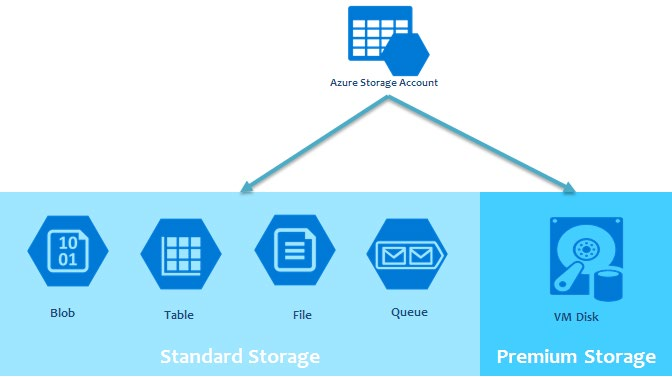
\includegraphics[width=0.6\textwidth]{azure-storage-account.png}
    \caption{Azure Storage account}
\end{figure}

\subsection{Azure Files}

\begin{itemize}
    \item  Hard Disk maar in de Cloud
    \item  Je kan deze mappen naar eigen pc, vb Z:\...
    \item  Handig als je veilig files wil kopiëren tussen Cloud server en on premise server
    \item  Zal de gekende protocollen volgen zoals SMB 3.0
    \item  Veel gebruikt in Hybrid Cloud
    \item  Werkt niet op school (Blocked)
    \item  Kan je thuis eens proberen
\end{itemize}

\begin{figure}[H]
    \centering
    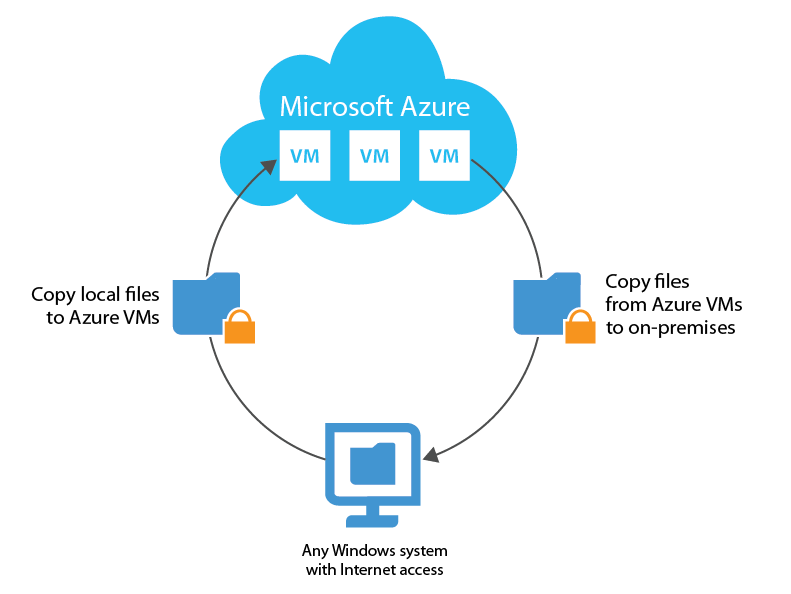
\includegraphics[width=0.6\textwidth]{azure-storage-files.png}
    \caption{}
\end{figure}


\subsection{Azure Disk Storage}

\begin{itemize}
    \item Basis voor Azure VM
    \item Op deze locaties komt de server te staan
    \item Ook mogelijkheid om datadisks te maken
    \item Hoge beschikbaarheid
    \item Lage latency
    \item Hoge throughput(2000MB/s)
    \item Mogelijkheid voor SSD disk
    \item Disk Encryption
    beschikbaar
\end{itemize}

\begin{figure}[H]
    \centering
    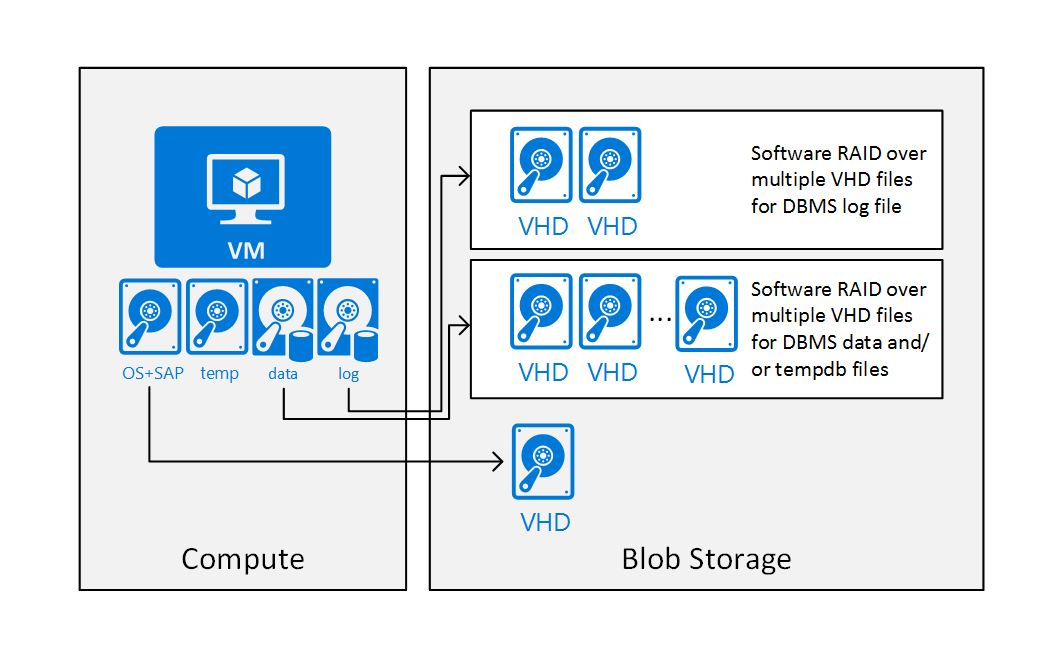
\includegraphics[width=0.6\textwidth]{azure-storage-disk.png}
    \caption{}
\end{figure}

\subsection{Azure Blob Storage}

\begin{itemize}
    \item `blob' == binary large object
    \item Opslag van bestanden: afbeeldingen, PDF, CSS, JS files van web apps kan je hier plaatsen
    \item Single page apps (Vue, Angular, Blazor)
    \item Container
    \begin{itemize}
        \item Bevat de bestanden
        \item Naam opgeven
        \item Public Access Level (wie kan welke bestanden lezen)
        \begin{enumerate}
            \item Private (default): extern bekijken is niet mogelijk
            \item Blob: extern lezen per blob is mogelijk
            \item Container: extern lezen van volledige container is mogelijk
        \end{enumerate}
    \end{itemize}
    \item Bestanden uploaden via storage explorer (\url{https://azure.microsoft.com/en-us/features/storage-explorer/})
    \item Connecteren met accountnaam/access key
    \item We kunnen bestanden opvragen via HTTP Request
\end{itemize}

\subsubsection{Pricing}

\begin{itemize}
    \item Prijs is per GB/per maand
    \item Hot of cool access
    \item We betalen ook de lees en schrijfoperaties
\end{itemize}

\begin{figure}[H]
    \centering
    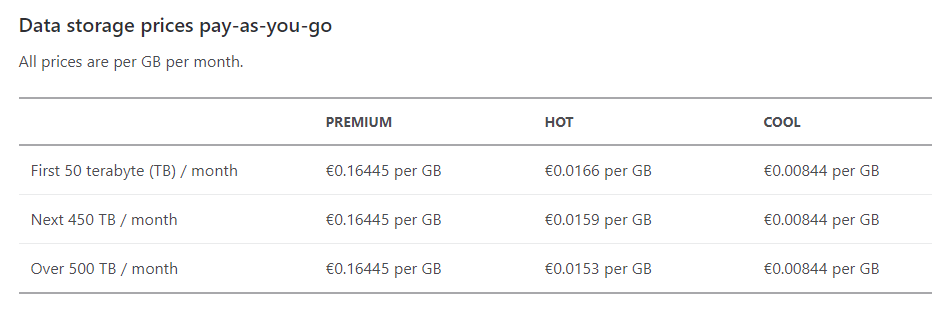
\includegraphics[width=0.6\textwidth]{azure-storage-blob-pricing.png}
    \caption{Prijstabel Azure Blob Storage}
\end{figure}

\subsubsection{Hot Access}

\begin{itemize}
    \item Data die nu in gebruik is en waar we veel lezen en schrijven
    \item Data die klaar staat om eventueel later naar cool storage te verplaatsen
\end{itemize}

\subsubsection{Cool Access}

\begin{itemize}
    \item Backups voor lange termijn
    \item Data die we niet frequent nodig hebben
\end{itemize}

\subsubsection{Static website}

\begin{itemize}
    \item Eenvoudige HTML website
    \item Ideaal voor VueJS, Angular, Reactor, Blazor, \dots
    \item Eventueel backend in Azure Functions en via JavaScript aangeroepen
    \item Zeer goedkoop
    \item \url{https://docs.microsoft.com/en-us/azure/static-web-apps/overview}
\end{itemize}

\subsection{Azure Storage Queues}

\begin{itemize}
    \item Een \bold{wachtrij} in de Cloud
    \item Een applicatie zal berichten op de wachtrij plaatsen (\bold{Sender})
    \item Een tweede applicatie kan deze berichten op een zelf gekozen moment ophalen en verwerken (\bold{Receiver})
    \item We spreken over een \bold{\underline{decoupled}} applicatie: zender en ontvanger werken onafhankelijk van elkaar
    \item Zeer schaalbaar voor meerdere queues op te starten
    \item \bold{Resilience}: buffer van berichten op queue zorgt ervoor dat er niks verloren gaat als back-end wegvalt
\end{itemize}

\begin{figure}[H]
    \centering
    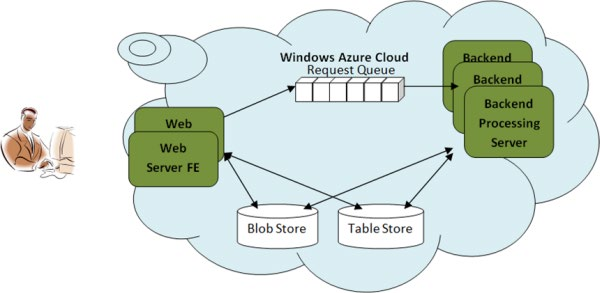
\includegraphics[width=0.6\textwidth]{azure-storage-queues.png}
    \caption{}
\end{figure}


\subsubsection{Voorbeeld}

\begin{itemize}
    \item Sender = webshop
    \item Ontvanger = stuk software (bv Azure Functions) die order zal controleren en naar een nieuwe wachtrij zal sturen
\end{itemize}

\begin{figure}[H]
    \centering
    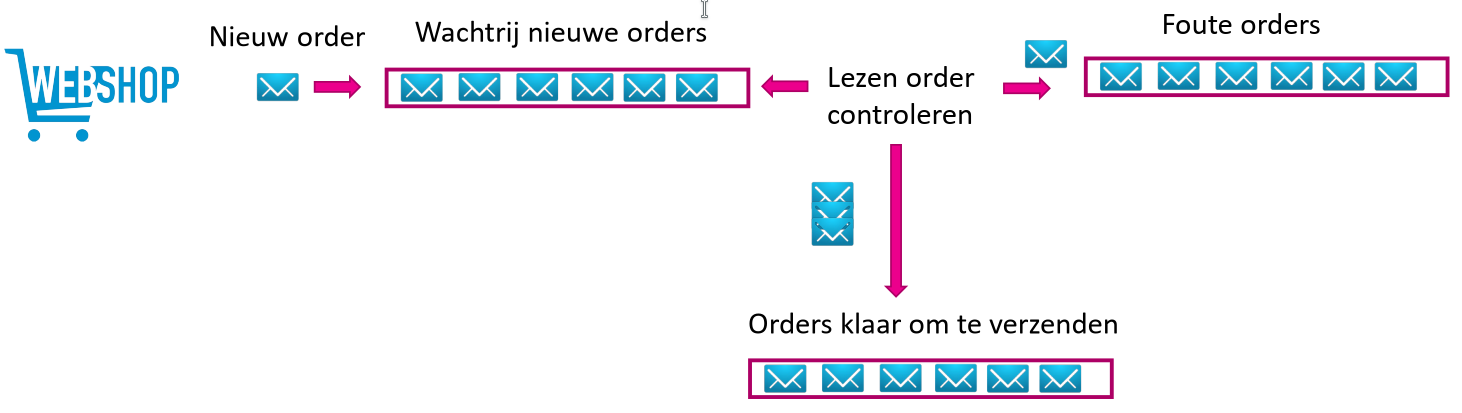
\includegraphics[width=0.5\textwidth]{azure-storage-queues-voorbeeld.png}
    \caption{}
\end{figure}

\subsubsection{Load leveling}

\begin{itemize}
    \item Constante load op applicatie die verwerkt moet worden
    \item Werkt zolang we niet meer berichten aanmaken dan wat de applicatie kan verwerken
\end{itemize}

\begin{figure}[H]
    \centering
    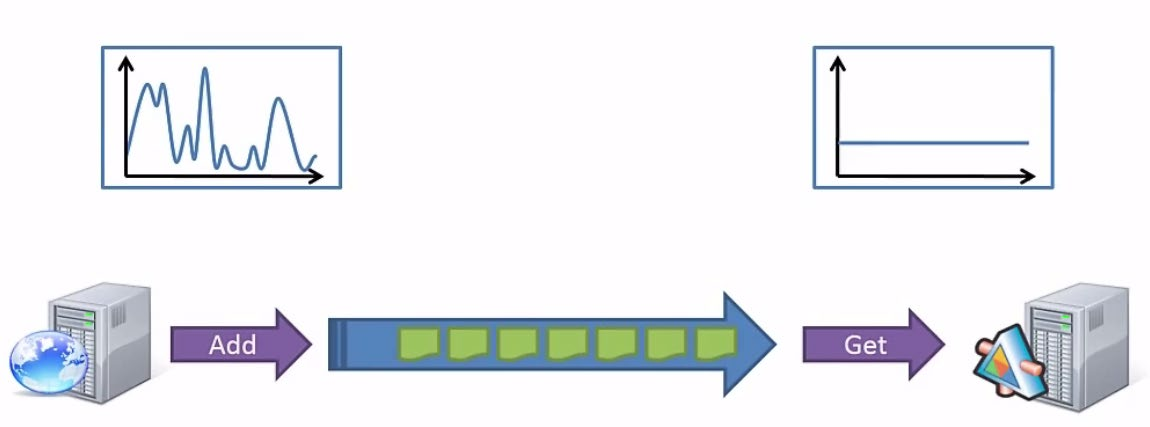
\includegraphics[width=0.5\textwidth]{load-leveling.png}
    \caption{}
\end{figure}

\subsubsection{Load balancing}

\begin{itemize}
    \item Teveel berichten per uur
    \begin{itemize}
        \item Applicatie die verwerkt schalen
        \item Nieuwe instantie $\Rightarrow$ verdubbeling verwerking
    \end{itemize}
    \item Wanneer terug minder berichten per uur: 1 applicatie stoppen
    \item High Availability $\Rightarrow$ bij crash 1 app, ligt systeem \bold{niet} plat
\end{itemize}

\begin{figure}[H]
    \centering
    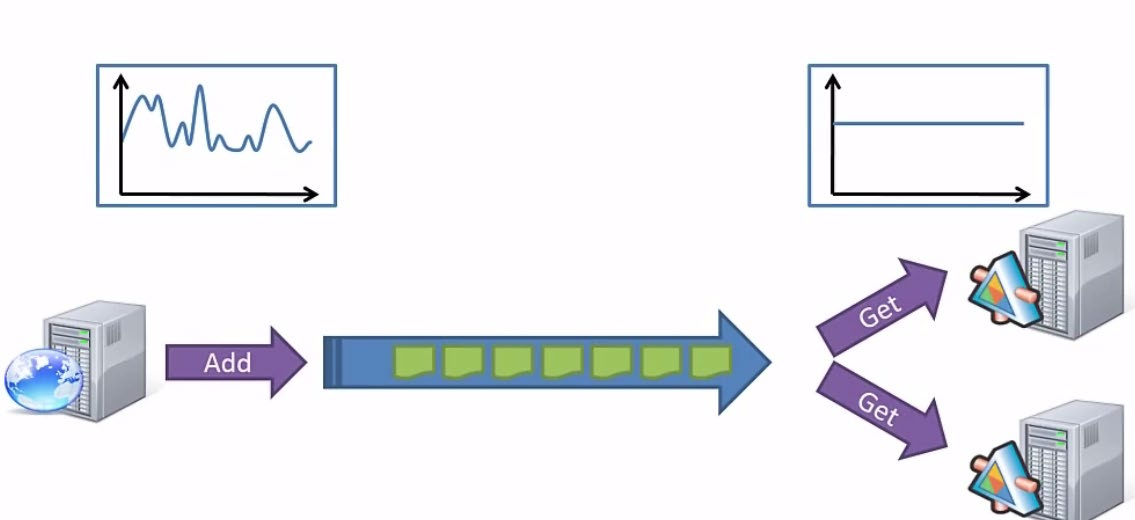
\includegraphics[width=0.5\textwidth]{load-balancing.png}
    \caption{}
\end{figure}

\subsubsection{Temporal decoupling}

\begin{itemize}
    \item We slaan alles op in Queue voor later
    \item Applicatie voor werking start om 23u op
    \begin{enumerate}
        \item Verwerkt alles
        \item Shutdown app
    \end{enumerate}
\end{itemize}

\begin{figure}[H]
    \centering
    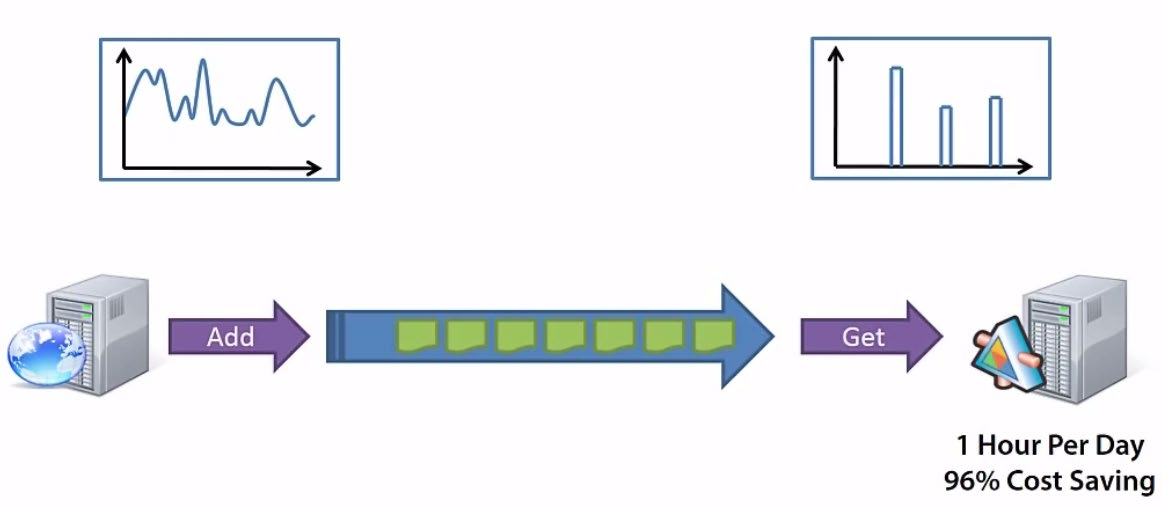
\includegraphics[width=0.5\textwidth]{temporal-decoupling.png}
    \caption{}
\end{figure}

\subsection{Azure Table Storage}

\begin{itemize}
    \item NO-SQL key/value store
    \item Opslag van Petabytes aan data
    \item Geo-redundant storage
    \item Flexibel dataschema, aantal kolommen per rij moet niet hetzelfde zijn
    \item Vergelijk het met een spreadsheet die je invult
    \item Geen relaties, geen joins, geen stored procedures
    \item Eenvoudig in gebruik
    \item Voorbeeld: \url{https://www.troyhunt.com/working-with-154-million-records-on/}
\end{itemize}

\begin{figure}[H]
    \centering
    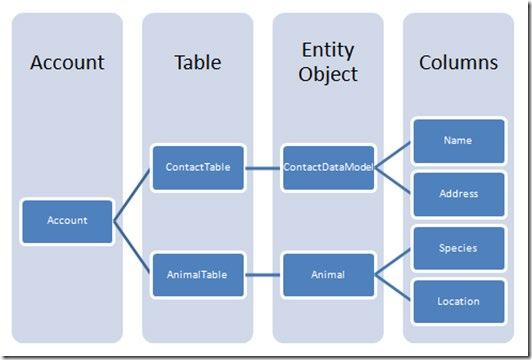
\includegraphics[width=0.5\textwidth]{azure-storage-table.png}
    \caption{}
\end{figure}

\begin{itemize}
    \item Partitions
    \begin{itemize}
        \item Verdelen van table over partities
        \item Iedere partitie op eigen server
        \item Zal beter schalen en load verdelen op server
    \end{itemize}
    \item Load balancing over 3 servers
    \begin{itemize}
        \item Azure zal data repliceren op 3 servers
        \item Verdelen van load over deze servers
    \end{itemize}
\end{itemize}

\begin{figure}[H]
    \centering
    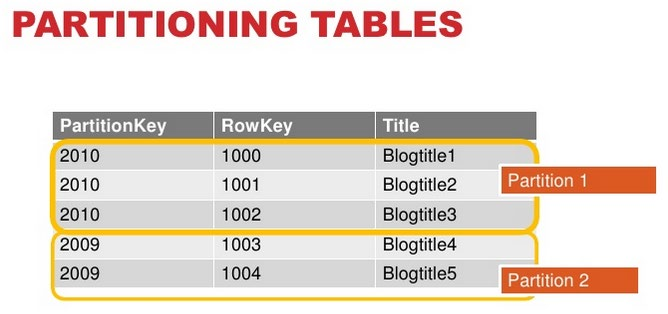
\includegraphics[width=0.5\textwidth]{partitioning-tables.png}
    \caption{}
\end{figure}

\subsubsection{Entities (rijen)}

\begin{itemize}
    \item Max 1MB
    \item 255 properties (kolommen), waarvan 3 verplicht:
    \begin{itemize}
        \item Parition key
        \item Row key
        \item Timestamp (automatisch)
    \end{itemize}
    \item Niet iedere rij moet evenveel kolommen hebben
\end{itemize}

\subsubsection{Table Storage Data Access}

\begin{itemize}
    \item Via REST API $\Rightarrow$ cross platform HTTP requests (.NET, PHP, Android, Objective C)
    \item Storage Client API (via Nuget Package Azure Storage)
    \item Voor andere platformen zijn er ook libraries (iOS, Android, Python, \dots)
\end{itemize}

\subsubsection{Queries}

\begin{itemize}
    \item Max 1000 items terugkeren
    \item Indien > 1000 $\Rightarrow$ Continuation token
    \item Query > 30 sec $\Rightarrow$ cancelled
    \item Geen index mogelijk
    \item Query op partition key \& row key $\Rightarrow$ snel
\end{itemize}

\subsubsection{Kolom types: }

\begin{itemize}
    \item Byte[] (=bytearray)
    \item Bool
    \item DateTime
    \item Double
    \item GUID
    \item Int32 of int
    \item Int64 of long
    \item String
\end{itemize}

\subsubsection{Waar gebruiken?}

\begin{itemize}
    \item Profiel info (zal niet veel wijzigen)
    \item Device info (bv: alle IMEI nummers van GSM toestellen binnen een netwerk)
    \item Telemetry data (bv: sensor netwerken die om de 5sec waarde van sensor doorsturen)
    \item Data voor AI modellen
    \item Alles waar je zeer veel niet-wijzigende data wenst op te slaan
\end{itemize}

\subsection{Azure Storage Tools}

Met behulp van de Storage Explorer: 

\url{https://azure.microsoft.com/en-us/features/storage-explorer/}

\subsection{Programmeren van Azure Storage}

\subsubsection{Wanneer?}

\begin{itemize}
    \item Opladen van bestanden op Blob storage
    \item Versturen van berichten naar wachtrijen (Queues)
    \item Wegschrijven van records naar Table Storage
\end{itemize}

Dit kan je allemaal programmeren via C\#, Python of JavaScript

\begin{itemize}
    \item In .NET Nuget Package toevoegen (zoals pip install bij Python)
    \item Rechtermuisknop op dependencies $\Rightarrow$ Manage Nuget packages
    \item Zoeken achter juiste package, vb: Azure Storage
\end{itemize}

\begin{figure}[H]
    \centering
    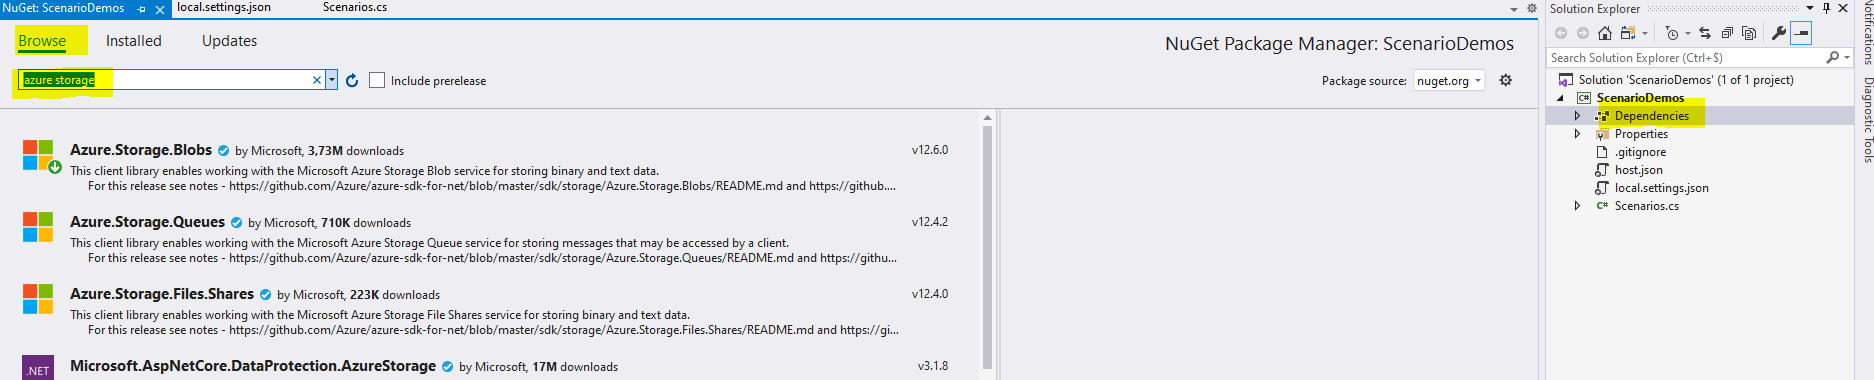
\includegraphics[width=0.5\textwidth]{azure-storage-visual-studio.png}
    \caption{Azure Storage toevoegen in Visual Studio 2019}
\end{figure}

\subsection{Enkele scenario's}

\subsubsection{Post binary file naar Azure Functions en opslag in op Azure Blob}

\begin{figure}[H]
    \centering
    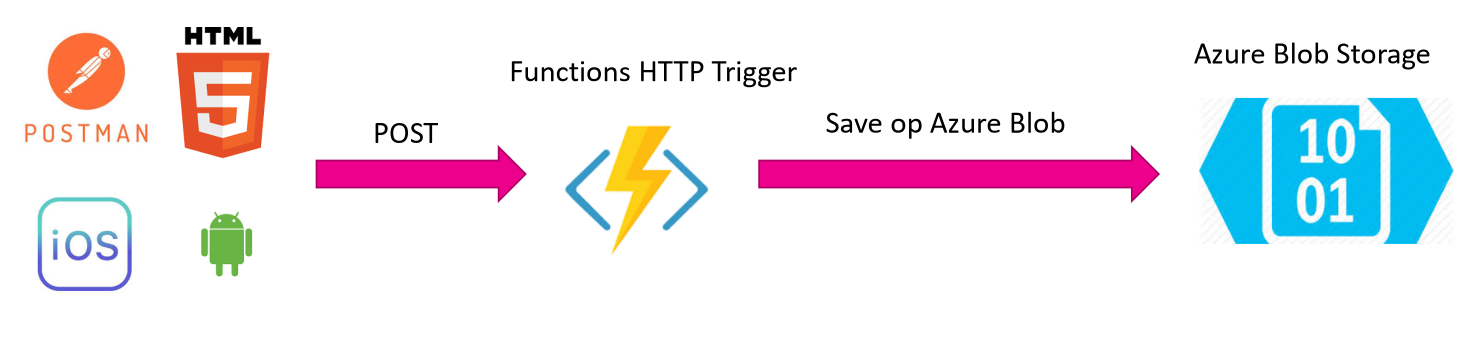
\includegraphics[width=0.5\textwidth]{azure-storage-scenario-1.png}
    \caption{POST binary file naar Azure Functions, opslag in Azure blob}
\end{figure}

\begin{figure}[H]
    \centering
    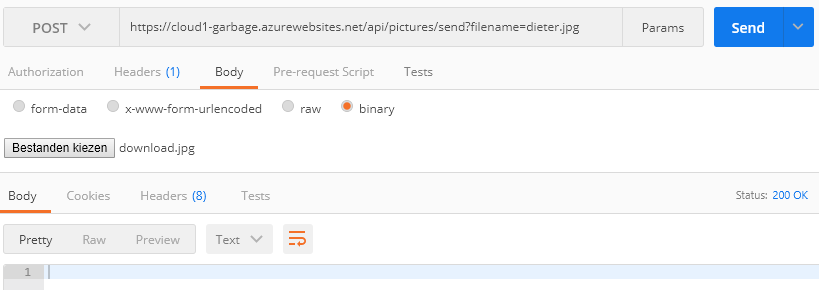
\includegraphics[width=0.5\textwidth]{scenario-1-1.png}
    \caption{De Binary data komt in de body van het HTTP Request via Postman}
\end{figure}

\begin{figure}[H]
    \centering
    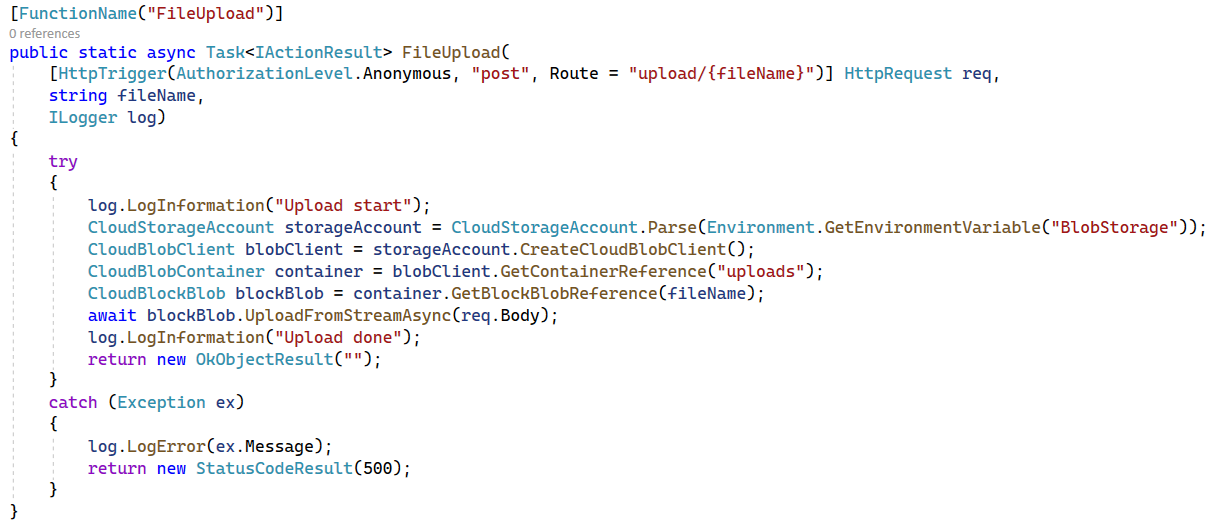
\includegraphics[width=0.5\textwidth]{scenario-1-2.png}
    \caption{Daarna slaan we de file op in de Blob Storage}
\end{figure}

\begin{figure}[H]
    \centering
    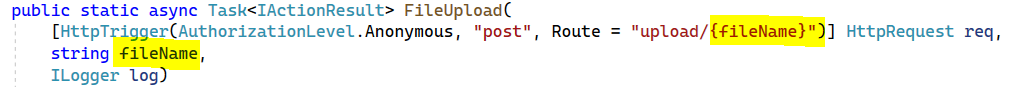
\includegraphics[width=0.8\textwidth]{scenario-1-3.png}
    \caption{Via de parameter in URL geven we de naam van het bestand mee aan service}
\end{figure}

\begin{figure}[H]
    \centering
    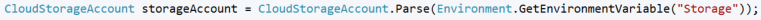
\includegraphics[width=0.9\textwidth]{scenario-1-4.png}
    \caption{Connectie maken met storage via connectiestring die we ophalen uit localsettings.json file (Connectiestring Storage staat op Azure)}
\end{figure}

\begin{figure}[H]
    \centering
    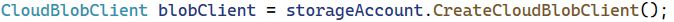
\includegraphics[width=0.3\textwidth]{scenario-1-6.png}
    \caption{Via CloudBlobClient kunnen we praten met de storage}
\end{figure}

\begin{figure}[H]
    \centering
    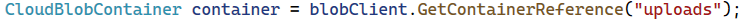
\includegraphics[width=0.7\textwidth]{scenario-1-7.png}
    \caption{We halen referentie op naar de container waar we de files willen opslaan}
\end{figure}

\begin{figure}[H]
    \centering
    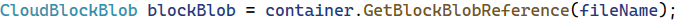
\includegraphics[width=0.7\textwidth]{scenario-1-8.png}
    \caption{We maken `lege' file aan}
\end{figure}

\begin{figure}[H]
    \centering
    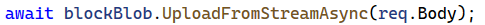
\includegraphics[width=0.7\textwidth]{scenario-1-9.png}
    \caption{We uploaden de stream van de body in de `lege' file}
\end{figure}

\subsubsection{Scenario 2}

\begin{figure}[H]
    \centering
    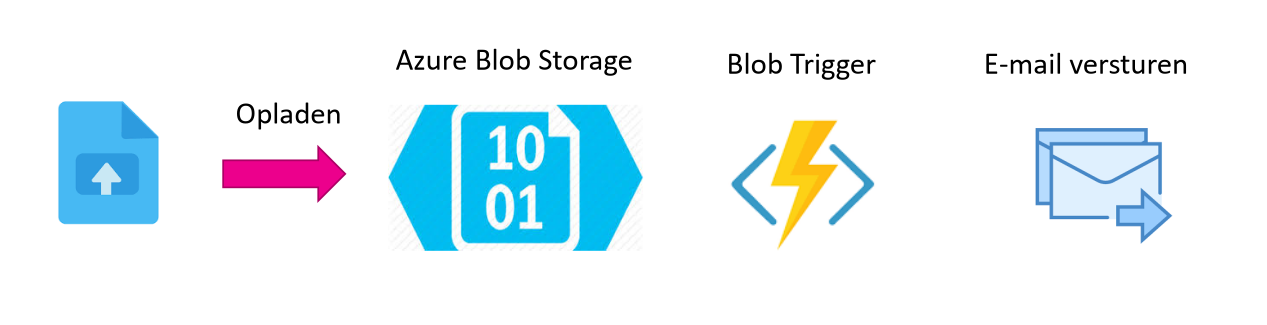
\includegraphics[width=0.5\textwidth]{azure-storage-scenario-2.png}
    \caption{Send e-mail wanneer een blob verschijnt op Azure Blob}
\end{figure}

\bold{Blob trigger}

\begin{itemize}
    \item Functie uitvoeren als er een Blob file aangemaakt is in een container
    \item Vb:
    \begin{itemize}
        \item Uploaden van foto's naar blob voor betere verwerking
        \item Uploaden CSV files voor verwerking
    \end{itemize}
\end{itemize}

\begin{figure}[H]
    \centering
    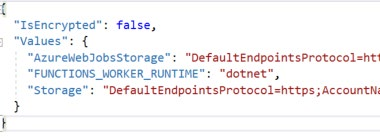
\includegraphics[width=0.5\textwidth]{scenario-2-1.png}
    \caption{In de settings file plaatsen we bij AzureWebJobStorage de connectionstring naar onze storage account}
\end{figure}

\begin{figure}[H]
    \centering
    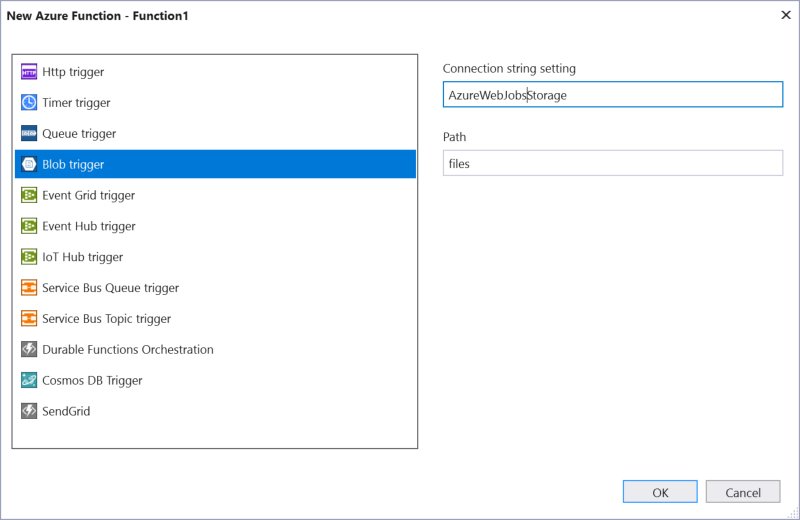
\includegraphics[width=0.5\textwidth]{scenario-2-2.png}
    \caption{Connectionstring = de key uit de settings file, Path = de naam van de container}
\end{figure}

\begin{itemize}
    \item Wat kunnen we doen met Blob?
    \begin{itemize}
        \item Sturen naar wachtrij
        \item Sturen naar Deep Learning netwerk voor training
        \item \dots
    \end{itemize}
    \item Dit voorbeeld: e-mail met link
    \item Hiervoor maken we gebruik van SendGrid en MailKit
\end{itemize}

\bold{SendGrid}

\begin{enumerate}
    \item In Azure Portal: nieuwe resource: `SendGrid Email Delivery'
    \item Kies voor het `Free' pricing tier
    \item SendGrid package: via Nuget Package manager in Visual Studio 2019
\end{enumerate}

\begin{figure}[H]
    \centering
    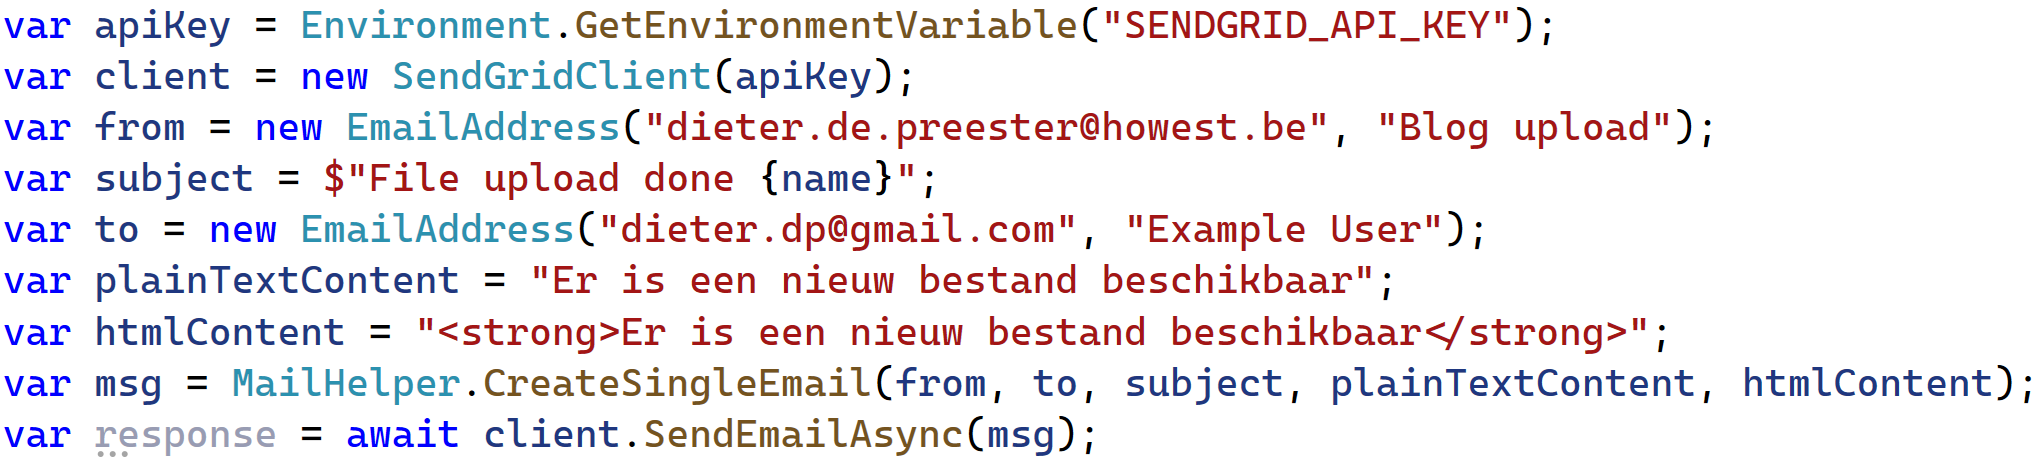
\includegraphics[width=0.5\textwidth]{scenario-2-3.png}
    \caption{API key nodig en plaatsen in config file Azure Functions}
\end{figure}


\bold{MailKit}

\begin{itemize}
    \item Alternatief voor SendGrid library (geen mailservice)
    \item Versturen van mails via Mailkit package
    \item SMTP mogelijkheden
\end{itemize}

\subsubsection{Scenario 3}

\begin{figure}[H]
    \centering
    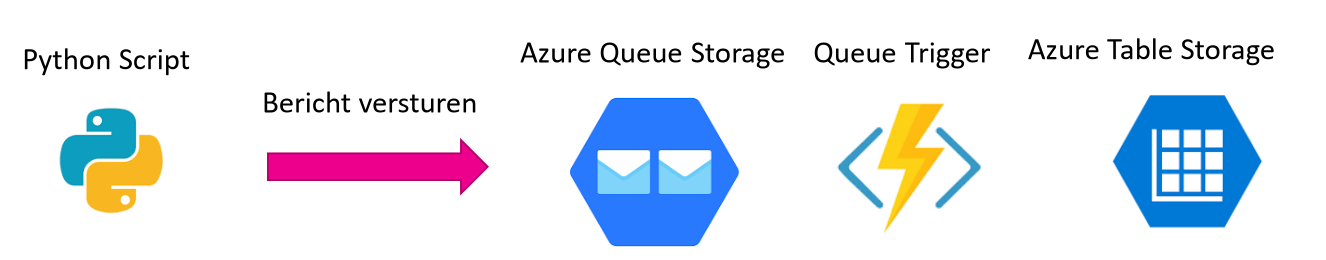
\includegraphics[width=0.5\textwidth]{azure-storage-scenario-3.png}
    \caption{We vullen een wachtrij voor verwerking door Azure Functions}
\end{figure}

\bold{Queue Trigger}

\begin{itemize}
    \item Functie zal actief worden bij ontvangst van een bericht op de Queue
    \item Ideaal voor het bufferen bij pieken
    \item Eenvoudig in gebruik
    \item In Visual studio: 
    \begin{itemize}
        \item Nieuwe Azure Function `Queue Trigger' met:
        \item Connectionstring = de connection key die bij de Queue storage hoort
        \item Queue name = naam van de wachtrij waarvan je berichten wenst te ontvangen
    \end{itemize}
\end{itemize}

\bold{Table Storage}

\begin{itemize}
    \item We ontvangen bericht en schrijven we naar Azure Table Storage
    \item We maken gebruik van de Nuget package `Microsoft.Azure.Cosmos.Table'
    \item We gaan temperatuur wegschrijven naar Azure Table Storage
\end{itemize}

\begin{figure}[H]
    \centering
    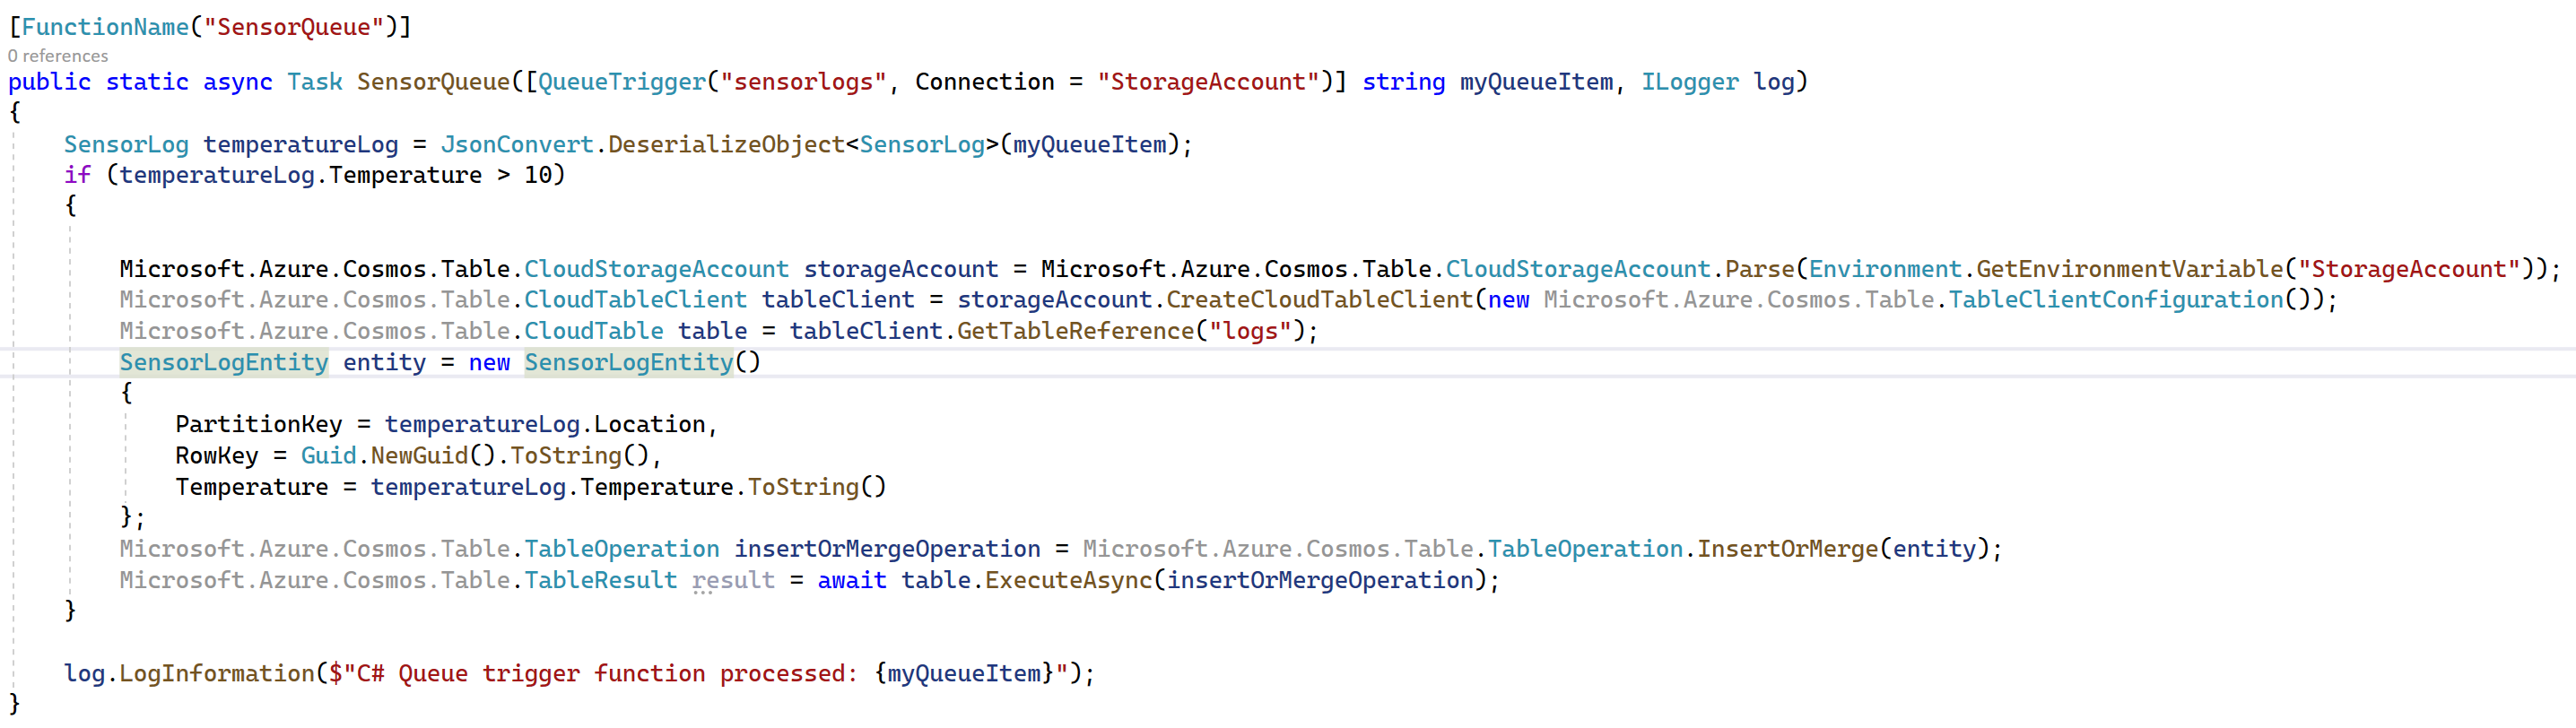
\includegraphics[width=0.75\textwidth]{scenario-3-1.png}
    \caption{Temperatuur wegschrijven naar Table Storage}
\end{figure}

\begin{figure}[H]
    \centering
    \includegraphics[width=0.4\textwidth]{scenario-3-2.png}
    \caption{Objecten voor Table Storage moeten erven van Table Entity}
\end{figure}

\bold{Hoe de Queue vullen? Meerdere mogelijkheden: }


\begin{itemize}
    \item Via website formulier
    \item Mobile app
    \item Python script via Raspberry Pi
    \item \dots
    \item \url{https://docs.microsoft.com/en-us/azure/storage/queues/storage-quickstart-queues-python}
\end{itemize}

\begin{figure}[H]
    \centering
    \includegraphics[width=0.5\textwidth]{scenario-3-3.png}
    \caption{Python script die queue opvult}
\end{figure}

\subsection{Good practices}

\begin{itemize}
    \item Iedere Azure Function heeft zijn eigen taak
    \item Veelgemaakte fout: 1 trigger die alles doet (bv: HTTP trigger die file upload doet en daarna ook mail verstuurt)
    \item Beter: HTTP trigger $\Rightarrow$ File naar Blob $\Rightarrow$ Blob Trigger $\Rightarrow$ Bericht op Queue $\Rightarrow$ Queue Trigger $\Rightarrow$ Mail sturen
    \begin{itemize}
        \item 3 triggers
        \item Schaalbaar
        \item Hogere performantie
    \end{itemize}
\end{itemize}

\subsection{Configuratiefiles lokaal of in de cloud?}

\begin{figure}[H]
    \centering
    \includegraphics[width=0.45\textwidth]{configuratie-lokaal.png}
    \includegraphics[width=0.45\textwidth]{configuratie-cloud.png}
    \caption{Lokaal (links) VS in de cloud (rechts)}
\end{figure}


\subsection{Samenvatting}

\begin{itemize}
    \item Welke zijn de verschillende soorten Azure Storage en wat is hun doel ?
    \item Wat is Azure Blob storage en wanneer gebruik je deze ?
    \item Wat is Azure Storage Queues en wanneer gebruik ik deze ?
    \item Wat is Azure Table Storage en wanneer gebruik ik deze ?
    \item Wat zijn partitions in Azure Table Storage ?
    \item Hoe werken Azure Functions Blob Triggers ?
    \item Waarvoor kan ik Azure Functions Blob Trigger gebruiken ?
    \item Wat is SendGrid ?
    \item Good practices
\end{itemize}

\section{MQTT}

= Message Queueing Telemetry Transport

= een machine-tot-machine (M2M) data transfer protocol die ons toelaat om berichten te sturen van een device naar een ander device.

\begin{figure}[H]
    \centering
    \includegraphics[width=0.7\textwidth]{mqtt.png}
    \caption{MQTT-broker}
\end{figure}

\subsection{Broker}

\begin{itemize}
    \item = software die instaat voor de communicatie volgens het MQTT protocol
    \item De broker staat centraal
    \item Doet niks anders dan berichten doorsturen en ontvangen
\end{itemize}

\subsubsection{Unmanaged services}

\begin{itemize}
    \item MQTT via eigen server
    \item Zowel VM als docker mogelijk
\end{itemize}

\subsubsection{Managed services}
\begin{itemize}
    \item Amazon IoT
    \item Google Cloud IoT
    \item Azure IoT Hub
\end{itemize}

\subsection{Doel}
\begin{itemize}
    \item Data verzamelen op device voor transport \bold{naar} cloud
    \item Data \bold{vanuit} de cloud naar de device sturen
    \item Communicatie tussen machines (M2M): vb tussen RPi, tussen Pi en ESP32, \dots
\end{itemize}

\subsection{Voordeel}
\begin{itemize}
    \item Lightweight (weinig overhead)
    \item Bi-directioneel (=two-way)
    \item Standaard (versie 3.1.1)
    \item Eenvoudig in gebruik
\end{itemize}

\subsection{Eigenschappen}

\begin{itemize}
    \item We spreken van een Publishing/Subscriber (Pub/Sub) protocol
    \item Centraal staat de broker die de bemiddeling doet tussen de clients
    \item 1/meerdere clients schrijven zich in (subscribe) voor een onderwerp of \bold{`Topic'}
    \item 1/meerdere clients kunnen een bericht plaatsen (publish) op een \bold{`Topic'}
    \item Topic = soort wachtrij
    \item Pub/Sub weten niks van elkaars bestaan af: geen IP, geen ports, geen locatie, \dots
    \item Pub/Sub moeten niet op hetzelfde moment actief zijn, kan \bold{disconnected} werken
\end{itemize}


\begin{figure}[H]
    \centering
    \includegraphics[width=0.8\textwidth]{mqtt-brokers.png}
    \caption{Mogelijke MQTT brokers die je kan gebruiken}
\end{figure}

\subsection{Sectoren}

\begin{itemize}
    \item Telemetry
    \item Automotive
    \item Smart phone
    \item Energy Monitoring (vb Flukso)
    \item Chat Applications
    \item Notification services
    \item LoRa Gateway (multitech)
    \item Facebook Messenger
    \item Olie \& Gas
\end{itemize}

\subsection{Topics}

Broker (server) heeft een \bold{Topic}/Subject
\begin{itemize}
    \item vb: /howest/b008/sensors/temperatuur
    \item Zelfde vorm als url
\end{itemize}

Devices hebben \bold{Subscription} op een of meerdere \bold{Topics}

\begin{figure}[H]
    \centering
    \includegraphics[width=0.7\textwidth]{mqtt-topics.png}
    \caption{Topic levels}
\end{figure}

\subsubsection{Wildcards}



\begin{figure}[H]
    \centering
    \includegraphics[width=0.6\textwidth]{mqtt-wildcards.png}
    \caption{Single-level wildcard: +}
\end{figure}


\begin{figure}[H]
    \centering
    \includegraphics[width=0.6\textwidth]{mqtt-wildcards2.png}
    \caption{Multi-level wildcard: \#}
\end{figure}

\subsection{Quality Of Service (QoS)}
= een overeenkomst tussen zender en ontvanger om te garanderen dat een bericht geleverd wordt.

3 niveau's: 
\begin{enumerate}
    \item Fire and forget
    \item Delivered at least once
    \item Delivered exactly once
\end{enumerate}

\subsubsection{Level 0: Fire and forget}

The sender tries with best effort to send the message and relies
on the reliability of TCP. No retransmission takes place.

\subsubsection{Level 1: Delivered at least once}

The receiver will get the message at least once. If the receiver
does not acknowledge the message or the acknowledge gets lost on the way, it will be
resent until the sender gets an acknowledgement. Duplicate messages can occur.

\subsubsection{Level 2: Delivered exactly once}

The protocol makes sure that the message will arrive exactly once
at the receiver. This increases communication overhead but is the best option when
neither loss nor duplication of messages are acceptable.

\subsection{Communicatie}

\subsubsection{Payload}
= Wat zit in het bericht?

\begin{itemize}
    \item Vrij te kiezen
    \item JSON
    \item XML
    \item CSV
    \item \dots
\end{itemize}

\subsubsection{Eigenschappen}

\begin{itemize}
    \item Geen standaard
    \item Nadeel is interoperability = samenwerking met andere systemen omdat er geen afspraken zijn rond inhoud
    \item Goede documentatie nodig
\end{itemize}

\subsubsection{Security}

Login/wachtwoord

\begin{itemize}
    \item Eenvoudig maar niet veilig
    \item Proberen te vermijden
\end{itemize}

TLS (zie 3MCT)
\begin{itemize}
    \item Voorkeur, meest veilige
    \item Beveiligen van communicatiekanaal
    \item Nadeel is dat je krachtiger IoT device nodig hebt voor encryptie, dus niet overal mogelijk
    \item \url{https://paolopatierno.wordpress.com/2015/08/18/gnatmq-and-ssltls-support-make-it-up-and-running/}
\end{itemize}

\subsection{MQTT Tools}

MQTT.FX of MQTT Lens of MQTT Box (Windows Store) installeren om de broker te testen.

\begin{figure}[H]
    \centering
    \includegraphics[width=0.5\textwidth]{mqtt-tools.png}
    \caption{MQTT Tools}
\end{figure}

\subsection{MQTT.NET \& Python}

Met MQTT library voor .NET (Nuget package downloaden in Visual Studio)

\subsubsection{In C\#}

\begin{figure}[H]
    \centering
    \includegraphics[width=0.8\textwidth]{mqtt-net1.png}
    \caption{Connectie maken}
\end{figure}

\begin{figure}[H]
    \centering
    \includegraphics[width=0.7\textwidth]{mqtt-net2.png}
    \caption{Versturen bericht}
\end{figure}

\begin{figure}[H]
    \centering
    \includegraphics[width=0.7\textwidth]{mqtt-net3.png}
    \caption{Ontvangen bericht via een Event}
\end{figure}

\begin{figure}[H]
    \centering
    \includegraphics[width=0.8\textwidth]{mqtt-net4.png}
    \caption{Meerdere topic publishen}
\end{figure}

\begin{figure}[H]
    \centering
    \includegraphics[width=0.85\textwidth]{mqtt-net5.png}
    \caption{Receive (met multi-level wildcard \#)}
\end{figure}

\subsubsection{In Python}

\begin{figure}[H]
    \centering
    \includegraphics[width=0.9\textwidth]{mqtt-python.png}
    \caption{}
\end{figure}

\subsection{MQTT en Azure Functions}

De MQTT Broker kan Azure Function Triggers activeren met de Nuget Extension:

`CaseOnline.Azure.WebJobs.Extension.Mqtt'

\url{https://github.com/keesschollaart81/CaseOnline.Azure.WebJobs.Extensions.Mqtt}

\begin{figure}[H]
    \centering
    \includegraphics[width=0.85\textwidth]{mqtt-azurefunction.png}
    \caption{MQTT Azure Function}
\end{figure}

\subsubsection{Opstellingen}

\bold{Directe communicatie} (one-way)

\begin{itemize}
    \item Vanuit App direct communiceren met MQTT broker via internet
    \item Voor de meeste platformen (iOS, Android, Windows is dit mogelijk)
    \item Niet altijd beste oplossing (poorten niet altijd open)
\end{itemize}

\begin{figure}[H]
    \centering
    \includegraphics[width=0.7\textwidth]{mqtt-com1.png}
    \caption{}
\end{figure}


\bold{Bericht via Azure Function naar MQTT} (one-way)

\begin{itemize}
    \item Vanuit App HTTP POST naar Azure Functions
    \item In de Azure function maken we bericht aan om te versturen naar MQTT Broker Topic
\end{itemize}

\begin{figure}[H]
    \centering
    \includegraphics[width=0.7\textwidth]{mqtt-com2.png}
    \caption{}
\end{figure}

\bold{Communicatie tussen devices via de cloud}

Als we op een drukknop aangesloten aan de RPI drukken: 
\begin{itemize}
    \item Publish bericht in /howest/gkg/b008/\#
    \item Broker draait in Cloud
    \item Iedereen met subscription op /howest/gkg/b008/\# zal dit ontvangen
\end{itemize}

\begin{figure}[H]
    \centering
    \includegraphics[width=0.7\textwidth]{mqtt-com3.png}
    \caption{}
\end{figure}

\bold{Communicatie tussen devices lokaal (zonder cloud)}

\begin{itemize}
    \item We kunnen de MQTT broker installeren op de Raspberry Pi
    \item Devices connecteren met elkaar via de lokale browser op de Pi
    \item Geen link met de cloud nodig
\end{itemize}

\begin{figure}[H]
    \centering
    \includegraphics[width=0.7\textwidth]{mqtt-com4.png}
    \caption{}
\end{figure}

\bold{Communicatie tussen devices lokaal via gateway met cloud link}

\begin{itemize}
    \item We kunnen een MQTT Broker installeren op de Raspberry Pi
    \item Devices communiceren met elkaar via de lokale broker op de Pi
    \item Via een mobile app sturen we bericht naar Azure Function LED AAN
    \item Function plaatst bericht in Topic /howest/gkg/b008/\#
    \item Vraagt VPN (complex)
\end{itemize}

\begin{figure}[H]
    \centering
    \includegraphics[width=0.7\textwidth]{mqtt-com5.png}
    \caption{}
\end{figure}

\subsection{Samenvatting}

\begin{itemize}
    \item Wat is MQTT ?
    \item Wat zijn topics \& subscriptions ?
    \item Welke vormen van topics zijn er, Wilcards etc
    \item Wat is QoS en welke zijn er ?
    \item Welke opstellingen zijn er mogelijk ?
\end{itemize}

\section{IoT Hub}

Azure IoT Hub is a fully managed service that enables \bold{reliable} and \bold{secure}
\bold{bidirectional communications} between millions of IoT devices and a
\bold{solution back end}

\begin{itemize}
    \item Managed Service: we moeten niks installeren in de cloud
    \item Bi-Directional Communication
    \item \bold{Miljoenen} toestellen
    \item Support voor meerdere talen (C\#,Python,C,Node)
    \item HTTPS/AMQP/MQTT protocol support
    \item Versturen telemetrie data $\Rightarrow$ Device To Cloud
    \item Ontvangen van commands $\Rightarrow$ Cloud To Device
    \item Beheer van devices via digital twin
    \item Queries op devices
    \item End-to-end security
    \item Certificaten per device
    \item TLS support
    \item X,509 support
    \item IP Whitelisting/blacklisting van devices
    \item Firmware/software update support
    \item Eenvoudiger dan bij MQTT
\end{itemize}

\subsection{Werking}

\begin{itemize}
    \item Device zal rechtstreeks communiceren met IoT Hub
    \begin{itemize}
        \item Device To Cloud (D2C)
        \item Cloud To Device (C2D)
    \end{itemize}
    \item 3 Protocollen mogelijk:
    \begin{itemize}
        \item AMQP
        \item MQTT (beperkingen t.o.v. eigen MQTT Server)
        \item HTTPS
    \end{itemize}
    \item Meest eenvoudige opstelling
    \item Hardware moet wel krachtig genoeg zijn
\end{itemize}

\subsubsection{Wat als device niet krachtig genoeg is?}

\begin{itemize}
    \item Bv: Arduino, Mbed Cortex M0,M1, \dots (= "Leaf device")
    \item Goedkope hardware maar niet altijd direct mogelijk om te connecteren op het internet
\end{itemize}

\bold{Oplossing:}
\begin{itemize}
    \item Field gateway
    \item Kan Raspi zijn, maar ook industriele PC
    \item Krachtig genoeg om veilig met het internet te communiceren
    \item Field gateway zal lokaal met de minder krachtige device praten via CoAP, Bluetooth, AllJoyn, \dots
\end{itemize}

\begin{figure}[H]
    \centering
    \includegraphics[width=0.5\textwidth]{iot-hub.png}
    \caption{Bovenaan: rechtstreeks communiceren met IoT client, onderaan: via Field gateway naar minder krachtige devices}
\end{figure}



\begin{figure}[H]
    \centering
    \includegraphics[width=0.5\textwidth]{iot-leaf.png}
    \caption{Opstelling Field gateway}
\end{figure}

\bold{D2C:} Low powerd device zal communiceren met Raspi (Gateway)
Gateway zal data doorsturen naar Cloud

\bold{C2D:} IoT hub zal commando sturen naar Raspi (Gateway). Raspi zal commando
naar juiste device sturen

\subsection{Hoe data verwerken die binnenkomt op IoT Hub?}


\begin{itemize}
    \item Streaming analytics
    \item Message Queues
    \item Azure Functions
    \begin{itemize}
        \item Ontvangen van berichten
        \item Versturen van berichten (commando) naar IoT Hub
    \end{itemize}
\end{itemize}

\begin{figure}[H]
    \centering
    \includegraphics[width=0.5\textwidth]{iot-hub-trigger.png}
    \caption{Schematische voorstelling}
\end{figure}


\subsection{IoT Hub Device Twin}

\bold{Probleemstelling:} 

We hebben 10.000 toestellen verbonden met Azure IoT Hub. Deze toestellen sturen een
motor aan. Het aantal RPM zit vast in het Python script vb. 5000.
We willen aanpassing sturen naar 5000 toestellen.

Hoe kunnen we dit gaan doen ?

\bold{Oplossing: IoT Hub Device Twin}

\begin{itemize}
    \item Digitale "tweeling" van device in de cloud
    \item Ideaal om \bold{configuratie} naar een toestel te sturen
    \item Configuratie zal opgeslagen en gesynchroniseerd worden
    \begin{itemize}
        \item In de cloud (IoT Hub)
        \item Op het toestel (developer moet dit doen in Python)
    \end{itemize}
\end{itemize}

\bold{Voorbeelden}

\begin{itemize}
    \item We wensen enkel temperaturen boven een bepaalde waarde te loggen
    \item Instellen van parameter tijdstip van doorsturen
    \item Alles wat configureerbaar moet zijn op afstand
\end{itemize}

\textcolor{red}{Dit is een belangrijk verschil met MQTT, daar hebben we deze infrastructuur NIET. We
moeten dit zelf maken door berichten te sturen naar toestel en omgekeerd}

\subsubsection{Reporting properties}

\begin{itemize}
    \item Device kan rapporteren aan cloud
    \item Status van batterij
    \item Status van toestel
    \item Laatste keer upload van toestel naar cloud
    \item \dots
\end{itemize}

\begin{figure}[H]
    \centering
    \includegraphics[width=0.6\textwidth]{iot-device-twin.png}
    \caption{}
\end{figure}

\begin{figure}[H]
    \centering
    \includegraphics[width=0.7\textwidth]{iot-device-twin2.png}
    \caption{Properties opvragen en rapporteren in JSON}
\end{figure}

\subsubsection{Device methodes}

\begin{itemize}
    \item Methodes op toestel activeren en dit vanop afstand
    \item We gaan de effectieve Python methode vanop afstand starten
    \item Vb: Reboot toestel
    \item Via portal kunnen we de methode activeren
    \item Via C\# kunnen we de methode activeren
    \item Parameters meesturen ook mogelijk
    \item Opslaan van device info in JSON document
    \item Query's mogelijk: vb: SELECT alle devices WHERE batterijstatus > 10\%
\end{itemize}

\begin{figure}[H]
    \centering
    \includegraphics[width=0.5\textwidth]{iot-hub-device-direct-method-portal.png}
    \caption{In Azure Portal de methode activeren met een payload}
\end{figure}


\subsection{IoT Hub Trigger voor Azure Functions}

In Visual Studio: 

\begin{itemize}
    \item Opgeven connectiestring uit local settings
    \item Path $\Rightarrow$ default laten staan
    \item Data = array van bytes $\Rightarrow$ omzetten naar string (JSON)
\end{itemize}

\subsection{Ondersteuning}

\subsubsection{SDK's}

\begin{itemize}
    \item Java 
    \item Python
    \item NodeJS
    \item Microsoft .NET
    \item C
\end{itemize}

\subsubsection{Devices}

\begin{itemize}
    \item Raspberry Pi
    \item Arduino
    \item Intel Edison
    \item MXCHIP
    \item Sparkfun electronics
    \item Adafruit
    \item Particle
\end{itemize}

\subsection{IoT Edge}

= service \bold{bovenop} IoT Hub

\subsubsection{IoT Hub issues:}

\begin{itemize}
    \item Alles moet naar de cloud voor verwerking, niks lokaal, soms veel datatrafiek
    \item We zijn afhankelijk van het Internet
    \item Het is moeilijk om scripts op een device te updaten
    \item Script vraagt soms speciale libraries op devices, soms probleem om te installeren
    \item Versie beheer is lasting, welke device heeft welke software staan?
    \item Soms wil je bepaalde dat NIET naar Cloud sturen (mag bedrijf niet verlaten)
\end{itemize}

\subsubsection{Doelstelling}

\begin{itemize}
    \item Cloud workloads lokaal draaien
    \item Eerste filtering van data op device doen
    \item Niet alles doorsturen naar Cloud
    \item Offline scenario voorzien
    \item Kosten in de cloud dalen
    \item Makkelijk updaten van IoT Edge device
\end{itemize}

\subsubsection{Voorbeelden}

\begin{itemize}
    \item Foto analyse op IoT Edge $\Rightarrow$ we moeten foto niet naar Cloud sturen voor analyse
    \item Filteren van data op de Edge Device
    \item Lokale data opslag
\end{itemize}

\subsubsection{Opbouw}

\begin{figure}[H]
    \centering
    \includegraphics[width=0.8\textwidth]{iot-edge2.png}
    \caption{IoT Edge draait op Docker. Modules zijn Docker Containers}
\end{figure}

\subsubsection{Azure IoT Edge Runtime}

\begin{itemize}
    \item Draait op bv RPi of industriele PC
    \item Installatie van workloads \& update op device
    \item Beveiligen van Edge communicatie
    \item Verantwoordelijk voor het uitvoeren van de modules
    \item Status health rapporteren aan de Cloud voor remote monitoring
    \item Zal zorgen voor communicatie met Leaf devices (low power toestellen zonder Internet)
    \item Zorgt voor communicatie tussen IoT Edge en modules op de device
    \item Zorgt voor communicatie tussen IoT Edge en Cloud
\end{itemize}

\begin{figure}[H]
    \centering
    \includegraphics[width=0.5\textwidth]{iot-edge3.png}
    \caption{}
\end{figure}

\subsubsection{Modules}

\begin{itemize}
    \item Functionaliteit toevoegen op de Edge
    \item Iedere module zal een actie uitvoeren
    \item We koppelen modules aan elkaar als een soort data processing pipeline
    \item We kunnen modules schrijven in C\#, Python, \dots
    \item Modules zijn Docker containers
\end{itemize}

\begin{figure}[H]
    \centering
    \includegraphics[width=0.5\textwidth]{iot-edge4.png}
    \caption{}
\end{figure}

\bold{Voorbeelden:}

\begin{enumerate}
    \item Module die data filtert voor deze naar de cloud te sturen
    \item Module die data omzet van XML naar JSOn voor deze naar de cloud te sturen
\end{enumerate}

\subsection{IoT in de Cloud vs IoT on the edge}

\subsubsection{IoT in the cloud}

\begin{itemize}
    \item Remote monitoring and control
    \item Merging remote data from across multiple IoT devices
    \item Near infinite compute and storage to train machine learning and other advanced AI tools
\end{itemize}

\subsubsection{IoT on the Edge}

\begin{itemize}
    \item Low latency tight control loops require near real-time response
    \item Public internet inherently unpredictable
    \item Privacy of data and protection of IP
\end{itemize}

\subsection{Samenvatting}

\begin{itemize}
    \item Wat en waarom IoT hub ?
    \item Waar zijn digitale twins bij IoT Hub en wat zijn de voordelen ?
    \item Wat zijn direct methods en wanneer gebruiken we dit ?
    \item Wat is IoT Edge ?
    \item Wanneer gebruiken we IoT Edge en wanneer IoT Hub ?
\end{itemize}

\section{Azure CosmosDB}

\subsection{Relationele databases}

= Opslag van data op gestructureerde manier

\begin{itemize}
    \item We slaan data op in verschillende tabellen
    \begin{itemize}
        \item Via normalisatie bepalen we de tabellen die we nodig hebben
        \item We stellen schema op waarin de data moet passen
    \end{itemize}
    \item Een tabel bestaat uit
    \begin{itemize}
        \item Rijen (record), die de data voorstellen
        \item Kolommen (welke info slaan we op)
    \end{itemize}
    \item We kunnen tabellen met elkaar verbinden via relaties
    \begin{itemize}
        \item We maken hiervoor gebruik van vreemde sleutels (kolom die zal verwijzen naar record in een andere tabel
    \end{itemize}
    \item We maken gebruik van de taal SQL voor
    \begin{itemize}
        \item Data opvragen (SELECT)
        \item Data toevoegen (INSERT)
        \item Data wijzigen (UPDATE)
        \item Data verwijderen (DELETE)
    \end{itemize}
    \item Via DDL kunnen we tabellen aanmaken (CREATE TABLE), \dots
    \item Wij kennen:
    \begin{itemize}
        \item SQL Database (Op Azure)
        \item MySQL Lokaal op de RPi maar ook op de Azure Cloud
    \end{itemize}
\end{itemize}

\subsubsection{Waarom ontstaan?}

\begin{itemize}
    \item Ontstaan in client/server periode
    \item Er was nog geen sprake van Internet, Cloud, Mobile data etc \dots
    \item Was vooral gemaakt om op 1 server te werken, meestal centraal in bedrijf
    \item Enige manier om te schalen was krachtiger CPU/Network/Storage $\Rightarrow$ Scale up
    \item \bold{Opgepast:} blijft zeer belangrijk binnen bedrijven, veel software moet integreren met bestaande systemen waaronder SQL
\end{itemize}

\subsection{NoSQL databases}

= `Non-SQL' of `non-relational SQL'

\begin{itemize}
    \item Databases die gemodelleerd zijn zonder tabelrelaties te gebruiken
\end{itemize}

\subsubsection{Waarom?}

\begin{itemize}
    \item Hoeveelheid data neemt enorm toe jaar na jaar
    \begin{itemize}
        \item Social Networks
        \item IoT Devices
        \item AI (Artificial Intelligence) \& Deep Learning systemen
    \end{itemize}
    \item Concurrency: veel gebruikers op hetzelfde moment: 10000 tot miljoenen
    \item Globaal bereikbaar en responsive
    \item Connectivity: veel gebruikers maar ook toestellen schrijven nu data weg of moeten data kunnen lezen
    \item Kan verschillende soorten data opslaan, structured,semi-structured en unstructured data
    \item Horizontal scaling, we kunnen eenvoudige meerdere servers toevoegen
\end{itemize}

$\Rightarrow$ \bold{Bovenstaande zaken zijn niet altijd mogelijk met relationele databases}

\subsubsection{Scaling}

\begin{itemize}
    \item Met eenvoudige hardware kunnen we scale-out doen door gewoon servers bij te plaatsen
    \item De hardware mag goedkoop zijn
    \item Geen downtime
    \item Eenvoudige te installeren en configureren
\end{itemize}

\begin{figure}[H]
    \centering
    \includegraphics[width=0.6\textwidth]{nosql-cost.png}
    \caption{Relationele DBMS vs NoSQL cost per concurrent user}
\end{figure}


\subsubsection{Availability and always-on}

\bold{Bij Relationeel (RDBMS)}


\begin{itemize}
    \item Gedeelde storage failure
    \item Volledige applicatie down
\end{itemize}

\begin{figure}[H]
    \centering
    \includegraphics[width=0.6\textwidth]{rdbms-availability.png}
    \caption{Beschikbaarheid bij RDBMS: single point of failure}
\end{figure}

\bold{Bij NoSQL}

\begin{itemize}
    \item Data zal op verschillende partities staan
    \item Geen gedeelde data
    \item Data zal naar alle storage weggeschreven worden, high availability (kan ook met RDBMS maar complex en extra software)
    \item We spreken hier over \bold{nodes}
\end{itemize}

\begin{figure}[H]
    \centering
    \includegraphics[width=0.6\textwidth]{nosql-availability.png}
    \caption{Beschikbaarheid bij NoSQL}
\end{figure}

\subsubsection{Global deployment}

\begin{itemize}
    \item Database in verschillende datacenters
    \item Zo dicht mogelijk bij de klant draaien latency zo < mogelijk
    \item Automatische replicatie van data tussen de verschillende datacenters
\end{itemize}

\begin{figure}[H]
    \centering
    \includegraphics[width=0.4\textwidth]{global-deployment.png}
    \caption{}
\end{figure}

\subsubsection{Gedistribueerde systemen}

\begin{itemize}
    \item NoSQL is een gedistribueerd systeem
    \item We hebben meerdere servers (we noemen dit ook soms nodes)
    \item Deze servers of nodes communiceren met elkaar over een netwerk
    \item Data zal op meerdere machines staan
    \item We merken dit niet, is transparant voor de applicatie
\end{itemize}

\subsection{Soorten NoSQL Databases}

\begin{enumerate}
    \item Key/Value (bv Azure table storage)
    \item Document database
    \item Column store (zien we niet)
    \item Graph (zien we niet)
\end{enumerate}

\subsubsection{Key/Value}

\begin{itemize}
    \item Meest eenvoudige NoSQL database
    \item Bestaat uit een unieke Key
    \item Voor iedere Key is er één waarde
    \item Value kan JSON zijn of ander document
    \item De NoSQL Database weet niet wat soort data het is, de database slaat enkel op, we moeten dus GEEN datatype opgeven
    \item De applicatie die data zal ophalen op basis van de Key moet de waarde kunnen interpreteren
\end{itemize}

\bold{Wanneer gebruiken?}

\begin{itemize}
    \item Sessie informatie gebruiker, user profiles, shoppint basket
    \item Data waar je minder moet in gaan zoeken via een query
    \item Data zonder relaties
\end{itemize}

\begin{figure}[H]
    \centering
    \includegraphics[width=0.5\textwidth]{key-value.png}
    \caption{Key-value database}
\end{figure}


\subsubsection{Document databases}

\begin{itemize}
    \item Basis is een document, geen record
    \item Het formaat is meestal JSON, maar XML of BSON (binary json) zijn ook mogelijk
    \item Het document zal zichzelf beschrijven, geen schema nodig zoals bij een SQL database
    \item Niet iedere document moet volgens hetzelfde schema zijn
    \item Er is een query taal om de data op te vragen en te doorzoeken
\end{itemize}

\bold{Wanneer gebruiken?}

\begin{itemize}
    \item Real-time analytics data
    \item IoT applications
    \item Vooral data die niet zoveel zal wijzigen, maar tegenwoordig meer en meer voor alle soorten data
\end{itemize}

\begin{figure}[H]
    \centering
    \includegraphics[width=0.6\textwidth]{document-database.png}
    \caption{Document Database}
\end{figure}

\subsubsection{Column store}

\begin{itemize}
    \item Dataopslag zal niet gebeuren op basis van records maar op basis van kolom
    \item Veel sneller bij zeer complexe query's
    \item Veel gebruikt voor data analyse systemen
\end{itemize}

\begin{figure}[H]
    \centering
    \includegraphics[width=0.6\textwidth]{column-store.png}
    \caption{Column store}
\end{figure}

\subsubsection{Graph Database}

\begin{itemize}
    \item Opslaan van entiteit en relaties tussen verschillende entiteiten
    \item Een entiteit is een soort node (object instantie) met properties
    \item Een relatie bevat ook properties vb: friend relation, project relation..
    \item De kracht zit in de relaties die je gaat opstellen tussen de entiteiten
\end{itemize}

\bold{Wanneer gebruiken?}

\begin{itemize}
    \item Social networking apps
    \item Spatial data apps
    \item Routing apps
\end{itemize}

\begin{figure}[H]
    \centering
    \includegraphics[width=0.6\textwidth]{graph-database.png}
    \caption{Graph database}
\end{figure}


\subsection{Voorbeeld SQL}

\begin{figure}[H]
    \centering
    \includegraphics[width=0.5\textwidth]{sql-normaliseren.png}
    \caption{Normaliseren van data naar tabellen voor gebruik in SQL}
\end{figure}

\begin{itemize}
    \item Normalisatie lukt wel maar blijft lastig
    \item Er zullen zaken bijkomen, vb. bedrijf, job role, \dots
    \item We moeten terug schema aanpassen
    \item We kunnen niet alles voorzien
    \item De data zit ook verspreid over de database $\Rightarrow$ complexe SELECT en JOIN nodig
    \item Full Text search is lastig, we moeten alles kolommen checken bij het zoeken
\end{itemize}

\subsection{Voorbeeld NoSQL}

\begin{itemize}
    \item Een record zal een document worden
    \item Makkelijk nieuwe velden toepassen
    \item Formaat is JSON
    \item We slaan data op als JSON in de database zelf
    \item We moeten data niet meer uitlezen en INSERT opbouwen
\end{itemize}

\bold{Nadeel}: dubbele data, geen relaties tussen data

\begin{figure}[H]
    \centering
    \includegraphics[width=0.3\textwidth]{nosql.png}
    \caption{Voorbeeld}
\end{figure}

\begin{figure}[H]
    \centering
    \includegraphics[width=0.5\textwidth]{nosql-techs.png}
    \caption{NoSQL technologie"en}
\end{figure}

\subsection{CosmosDB}

= CosmosDB is managed NoSQL database service op Azure

\begin{itemize}
    \item Geen onderhoud
    \item Geen patching
    \item Eenvoudige op te zetten
    \item Pay what you use
    \item Krachtige API's
\end{itemize}

\begin{figure}[H]
    \centering
    \includegraphics[width=0.5\textwidth]{cosmosdb.png}
    \caption{Azure Cosmos DB}
\end{figure}

\begin{itemize}
    \item Globaal gedistribueerde database
    \begin{itemize}
        \item Op eenvoudige manier de data zo dicht mogelijk bij de klant brengen
        \item Op eenvoudige manier activeren in datacenter dicht bij de gebruiker
        \item Geen complex configuratie voor nodig
    \end{itemize}
    \item Unlimited scalability
    \begin{itemize}
        \item Eenvoudig up- and down scaling wanneer je maar wilt
    \end{itemize}
    \item Low latency
    \item Meerdere data modellen en API's beschikbaar
    \begin{itemize}
        \item Document DB API
        \item MongoDB API
        \item Gremlin API
        \item \dots
        \item Zeer belangrijk bij het migreren van bestaande toepassingen naar CosmosDB
    \end{itemize}
    \item SLA
    \begin{itemize}
        \item Van 99,99\% in een region, meerdere regions = hogere SLA
    \end{itemize} 
\end{itemize}

\subsubsection{CosmosDB API}

\begin{itemize}
    \item Cosmos DB Account
    \item Database
    \begin{itemize}
        \item Groep die meerdere Containers (Collection) bevat
    \end{itemize} 
    \item Container == Tabel (in klassieke SQL)
    \begin{itemize}
        \item Bevat een verzameling van verschillende JSON documenten
    \end{itemize}
    \item Item == Record (in klassieke SQL)
    \begin{itemize}
        \item JSON content
    \end{itemize}
\end{itemize}

\begin{figure}[H]
    \centering
    \includegraphics[width=0.7\textwidth]{cosmosdb-api.png}
    \caption{}
\end{figure}

\subsubsection{CosmosDB API Account}

\begin{itemize}
    \item Wij gebruiken `SQL API'
    \item Capacity Node:
    \begin{itemize}
        \item Kies hier `serverless', we betalen enkel voor wat we gebruiken
        \item Kies `non production' om te testen
    \end{itemize}
\end{itemize}

\begin{figure}[H]
    \centering
    \includegraphics[width=0.6\textwidth]{cosmosdb-api-account.png}
    \caption{}
\end{figure}

\subsubsection{Kiezen van een API}

\begin{itemize}
    \item Bepalen bij aanmaak Account
    \item Je kan deze niet wijzigen achteraf
    \item Wij zullen SQL API gebruiken voor document databases
    \item \bold{Opgepast:} SQL API is niet zo krachtig als de SQL taal die we kennen
\end{itemize}

\begin{figure}[H]
    \centering
    \includegraphics[width=0.5\textwidth]{cosmosdb-api-choice.png}
    \caption{Kiezen van een API}
\end{figure}


\subsubsection{Container toevoegen}

= vergelijkbaar met de klassieke tabel uit RDBMS

\begin{itemize}
    \item Unieke database naam
    \item Unieke container naam (soort table)
    \item Partition Key (zelfs concept als table storage)
\end{itemize}

\begin{figure}[H]
    \centering
    \includegraphics[width=0.3\textwidth]{cosmosdb-addcontainer.png}
    \caption{}
\end{figure}

\subsubsection{Manueel data toevoegen}

\begin{figure}[H]
    \centering
    \includegraphics[width=0.7\textwidth]{cosmosdb-adddata.png}
    \caption{}
\end{figure}

\subsubsection{Firewall}

\begin{figure}[H]
    \centering
    \includegraphics[width=0.7\textwidth]{cosmosdb-firewall.png}
    \caption{}
\end{figure}

\subsubsection{Aanspreken vanuit Azure Functions met .NET}

\begin{itemize}
    \item Nuget Package: Microsoft.Azure.Cosmos
    \item 2 belangrijke parameters: URI en PRIMARY KEY
\end{itemize}

\begin{figure}[H]
    \centering
    \includegraphics[width=0.3\textwidth]{cosmosdb-parameters.png}
    \includegraphics[width=0.4\textwidth]{cosmosdb-localjson.png}
    \caption{}
\end{figure}

\bold{Stap 1: Connectie maken met CosmosDB}

\begin{itemize}
    \item CosmosClient object aanmaken met parameters uit local.settings.json
    \item Connectionstring meegeven
    \item ConnectionMode op Gateway (Alternatief is direct maar werkt niet in Howest)
\end{itemize}

\begin{figure}[H]
    \centering
    \includegraphics[width=0.8\textwidth]{cosmosdb-stap1.png}
    \caption{Verbinden met database via Environment Variables}
\end{figure}


\bold{Stap 2: Model van data die we wensen weg te schrijven}

\begin{itemize}
    \item {[JsonProperty]} gebruiken om lowercase property te bekomen in de database
    \item Id voorzien die uniek is
    \item PartitionKey moet ook aanwezig zijn in model
\end{itemize}

\begin{figure}[H]
    \centering
    \includegraphics[width=0.4\textwidth]{cosmosdb-stap2.png}
    \caption{Datamodel}
\end{figure}


\bold{Stap 3: Deserialisatie}

\begin{figure}[H]
    \centering
    \includegraphics[width=0.8\textwidth]{cosmosdb-stap3.png}
    \caption{Deserialisatie}
\end{figure}


\bold{Stap 4: Wegschrijven naar database}

\begin{itemize}
    \item Ophalen database en container waarnaar we wensen weg te schrijven
    \item Id invullen met unieke waarde
    \item CreateItemAsync aanroepen met model
\end{itemize}

\begin{figure}[H]
    \centering
    \includegraphics[width=0.8\textwidth]{cosmosdb-stap1.png}
    \caption{Wegschrijven van data}
\end{figure}


\bold{Stap 5: Bekijk data in Azure Portal of in Azure Storage Explorer}

\begin{figure}[H]
    \centering
    \includegraphics[width=0.5\textwidth]{cosmosdb-stap5-1.png}
    \includegraphics[width=0.3\textwidth]{cosmosdb-stap5-2.png}
    \caption{Azure Portal / Azure Storage Explorer}
\end{figure}

\bold{Stap 6: Opvragen van data}

\begin{figure}[H]
    \centering
    \includegraphics[width=0.6\textwidth]{cosmosdb-stap6.png}
    \caption{Opvragen van data}
\end{figure}

\subsubsection{CosmosDB extra's}

\begin{itemize}
    \item Azure Search
    \begin{itemize}
        \item Krachtige zoekmachine boven CosmosDB
        \item Text search
        \item Indexing
    \end{itemize}
    \item Azure Functions
    \begin{itemize}
        \item CosmosDB Trigger
        \item Bij toevoegen documenten $\Rightarrow$ functie activatie
    \end{itemize}
    \item Time To Live
    \begin{itemize}
        \item Automatisch verwijderen van items na x-aantal tijd
        \item Container niveau
        \item Item niveau
    \end{itemize}
\end{itemize}

\subsection{Extra's}

\begin{itemize}
    \item Stored Procedures
    \begin{itemize}
        \item Functies in de database
        \item Schrijven van complexe queries
        \item Werken op collection niveau
        \item Aanroepen via API of portal
        \item Javascript
    \end{itemize}
    \item UDF (User Defined Functions)
    \begin{itemize}
        \item Functies die we aanroepen vanuit queries
        \item Vb: berekening maken
        \item JS
    \end{itemize}
    \item \url{https://docs.microsoft.com/en-us/azure/cosmos-db/programming}
\end{itemize}

\begin{figure}[H]
    \centering
    \includegraphics[width=0.3\textwidth]{udf.png}
    \caption{Voorbeeld UDF aanmaken}
\end{figure}

\begin{figure}[H]
    \centering
    \includegraphics[width=0.6\textwidth]{udf2.png}
    \caption{UDF uitvoeren in query}
\end{figure}


\subsection{Samenvatting}

\begin{itemize}
    \item SQL vs NoSQL
    \item Waarom en wanneer NoSQL databases?
    \item Welke soorten NoSQL databases zijn er ?
    \item Weet hoe je kan lezen en schrijven naar CosmosDB ?
\end{itemize}

\section{Examen}
\begin{itemize}
    \item Theorie: 30\%
    \item Labo 70\%
    \item Het examen bevat zeker vragen over ofwel MQTT ofwel IoT
\end{itemize}

\end{document}